\documentclass{ifacconf}
\usepackage{graphicx}     
\usepackage{natbib}   
\usepackage{graphicx} % Required for inserting images
\usepackage{amsmath}
% \usepackage[french]{babel}
\usepackage{eurosym}
\usepackage{textcomp}
\usepackage{ulem}
\usepackage{subcaption}
\usepackage[utf8]{inputenc}
\usepackage{pgfplots}
\usepackage{xurl}
\usepackage{bm}
\DeclareUnicodeCharacter{2212}{−}
\usepgfplotslibrary{groupplots,dateplot}
\usetikzlibrary{patterns,shapes.arrows}
\pgfplotsset{compat=newest}
%\usepackage{appendix}


\begin{document}
\begin{frontmatter}
\title{Backcasting Policies in Transport Systems as an Optimal Control Problem : An Example with Electric Vehicle Purchase Incentives}

\author{Vinith Lakshmanan} 
\author{Xavier Guichet} 
\author{Antonio Sciarretta}

\address{IFP Energies Nouvelles, France (e-mail: vinith-kumar.lakshmanan@ifpen.fr, xavier.guichet@ifpen.fr, antonio.sciarretta@ifpen.fr).}
%\address[Second]{Department of Economic and Environmental Evaluation, 
  % IFP Energies Nouvelles, France (e-mail: xavier.guichet@ifpen.fr)}
%\address[Third]{Electrical Engineering Department, 
 %  Seoul National University, Seoul, Korea, (e-mail: author@snu.ac.kr)}

\begin{abstract}                % Abstract of not more than 250 words.
This study represents a first attempt to build a backcasting methodology to identify the optimal policy roadmaps in transport systems. Specifically, it considers a passenger car fleet subsystem, modelling its evolution and greenhouse gas emissions. The policy decision under consideration is the monetary incentive to the purchase of electric vehicles. This process is cast as an optimal control problem with the objective to minimize the total budget of the state and reach a desired CO$_2$ target. A case study applied to Metropolitan France is presented to illustrate the approach. Additionally, alternative policy scenarios are also analyzed.   
\end{abstract}

\begin{keyword}
Backcasting, Optimization, Policy-making, Transport system
\end{keyword}

\end{frontmatter}


\section{Introduction}

The European Union's (EU) goal of carbon neutrality by 2050 requires reducing transportation sector emissions by 90\% compared to 1990 levels. Transport alone is set to make up nearly half of Europe's greenhouse gas (GHG) emissions in 2030. Thus the European Commission has adopted a set of proposals to make the EU's policies fit for reducing net greenhouse gas emissions by at least 55\% by 2030 (\cite{GreenDeal}).
%
Similar targets are being implemented in U.S. and other regions (\cite{EPA}). 

Governance, policies, and incentives ("decisions") play an important role in shaping transport systems of the future, and influence the development and implementation of the various technologies and modes of transport. It is therefore important to study how decisions could be best used to govern transport systems in the desired direction of decarbonization. 

% \textit{In addition, the COVID-19 crisis has significantly altered commuting habits; remote and telework have become widespread together with other flexible work arrangements. The true impact of these changes on gas emissions and on the well-being of people as well as on the real-estate market (offices) are not known. This is now an opportunity to leverage on an ongoing change in habits that could result in significant GHG reduction.}

To find the best policy roadmaps for desired targets, the traditional approach consists in designing prospective scenarios, and testing them using simulation. Once the impacts are forecasted for each scenario, conclusions can be drawn on which decisions are the most effective. With this approach, the choice is limited to the scenarios designed, which may represent a tiny subset of all possibilities if multiple concurrent decisions are considered. Moreover, even when a small set of decisions are to be taken, the optimum might not be achieved since only the designed scenarios are evaluated.

To overcome these limitations, a backcasting paradigm is supported in this work. In this approach, desired targets are set by the decision makers at a certain time horizon, then the optimal combinations of policies to achieve these targets are calculated as a function of time (``backcasted"). 
In this way, the aprioristic choice of scenarios is replaced by a full dynamic optimization process that can explore among all combinations possible.

The backcasting paradigm has been introduced since the last century (\cite{Robinson, Bibri}). It has been mainly deployed in qualitative terms (\cite{Levitate}) or quantitatively with some static optimization procedure (\cite{Gomi, Ashina}).
However, this process can be more effectively cast as an optimal control problem, with a suitable definition of an objective function, an horizon, local and terminal constraints, etc.

 %However, with respect to the traditional approach, here the physical causality has to be somehow inverted.

%The availability of such a model thus represents the first step toward the new backcasting methodology. 
Clearly, since future impacts have to be predicted, the new backcasting paradigm is still based on a simulation model. This model must be able to describe transport as a system, with manipulable inputs, exogenous inputs or disturbances, outputs, and states. The manipulable inputs are represented by the decisions to optimize, which may concern local authorities, state government, EU, or even private companies. 
The exogenous inputs represent the influence of other, related systems such as the energy, urban, economic, demographic ones, which cannot be modeled within the transport system alone.
The outputs represent the impacts targeted or the constraints to impose to the backcasting process. Finally, the states are the dynamics associated with the internal variables. 

In this paper, we illustrate the backcasting paradigm, applied to the transport sector, by considering a specific subsystem with a single decision variable. The subsystem considered describes the evolution of the passenger car fleet within a certain region and its impacts on the GHG emissions. The decision optimized is a monetary incentive to the purchase of electric vehicles.

The prediction of vehicle fleet composition is the subject of a large body of literature (\cite{TREMOVE, High-Tool, ITF, ADEME}). Typically, dynamic fleet models are based on the evaluation of stocks and sales of various types of vehicles per time period. Stocks change in time due to disposal of old vehicles (due to scrappage, exports, change of use, etc.), and sales of new vehicles. The latter, in turn, are induced by transport demand (vkm) and mileage, and split among the vehicle types using discrete choice models (\cite{train, benakiva}). 

The GHG emissions of a given vehicle fleet are typically assessed using emission factors. CO$_2$ emissions of light-duty vehicles are regulated in the EU. Similar regulations are about to be applied to heavy-duty vehicles as well.
%Since 2021, new vehicles sold must emit at most 95~g(CO$_2$)/km. 

Recent studies that include electric vehicles have applied a fleet model to predict the future transport emissions in France (\cite{ADEME, ITF}), Norway (\cite{thorne}), Japan (\cite{sato}), and the U.S. (\cite{woody}).

The paper is organized as follows. Section~\ref{sec:model-refinement} introduces the passenger car fleet model, followed by the optimal control problem formulation. A case study, based on the French national passenger car fleet, is presented in Sect.~\ref{sec:casestudy}. The last section draws some conclusions and proposes several research directions to extend to a more realistic system model.

\section{Passenger Car Fleet Model} \label{sec:model-refinement}
This section presents the equations of the passenger car fleet model and the formulation of the proposed backcasting approach.  The latter consists in optimising some decisions concerning the transport system  in order to achieve some defined target in greenhouse-gas (CO$_2$) emissions at year $T$. We thus treat the transport system as a system having $\textbf{u}=
u_v(t)$ as the manipulable input to be backcasted in this study, where the monetary incentive to the purchase of electric vehicles (EV) given by the state ($u\equiv u_2$, while $u_1\equiv 0$), and the CO$_2$ emissions as the targeted output. 
% $\textbf{y}$. 
This system shall be represented by an aggregated dynamic model, which evaluates the transport emissions of the studied area as a function of time.

\subsection{Model}

We consider only a single area of interest and private car as the transport mode. In addition, we consider the latter's stock composed of two types of vehicles (thermal, $v=1$ and electric, $v=2$) differentiated by $A+1$ classes of ages ($a=0\ldots A$). We consider vehicle-km (vkm), a measure of transport demand $G(t)$, as an input provided by upstream models. Additionally, we also consider mileage $M(t)$ as an exogenous input.

We use one year as the time step and label the year index as $t$, starting from present until target year $T$. The passenger car fleet model can be written as follows. 

The demand of new vehicles $N$ at year $t$ is given by the ratio of the vkm demand for new vehicles, $F(t)$ and the mileage $M(t)$,
%
\begin{equation} \label{eqn:N}
  N(t) = \frac{F(t)}{M(t)}.
\end{equation}
%
The vkm demand for new vehicles is evaluated as the difference between total transport demand, $G(t)$ and those covered by the sum of the old vehicles disaggregated by vehicle type and age $O_{va}(t)$,
%
\begin{equation}\label{eqn:F2}
    F(t) = G(t) - M(t) \sum_{va} O_{va}(t)
\end{equation}
%
The latter is obtained using the age-dependant survival rate $\eta_a$ and the stock by vehicle type and age $S_{va}(t)$ at year $t$ as 
%
\begin{equation}\label{eqn:O2}
O_{va}(t) = \left\{ \begin{array}{ll} 
\eta_a S_{v,a-1}(t-1)  \quad \forall a=1,\ldots,A-1 \\  
\eta_A S_{v,A-1}(t-1) + \eta_A S_{vA}(t-1) 
\end{array} \right.
\end{equation}
%
% where $a'=a-1$.
The total sales at year $t$ are split among vehicle types according to 
%
\begin{equation} \label{eqn:Nv}
  N_v(t) = P_v(t)N(t),
\end{equation}
%
where $P_v$ is the share of sales by veh-type at year $t$. 

The latter is obtained from a logit expression
%
\begin{equation} \label{eqn:P}
  P_v(t) = \frac{e^{\mu U_v(t)}}{\sum_v e^{\mu U_v(t)} },
\end{equation}
%
where $U_v$ is the utility function by veh-type.

To evaluate the $P_v(t)$, we consider different technical-economic characteristics of the vehicles in its utility function, $U_v(t)$. Among the latter, we consider two classes of costs for the user: purchase costs, and operating costs (i.e., fuel/energy, maintenance, insurance costs). 
These are the main determinants for the choice of new vehicles. Another determinant is the development rate of the refilling (fuel/electricity) infrastructure which reflects its availability.
Conversely, we do not consider explicitly socio-economic determinants that depend on the single agent (like age, gender, income level, etc.) and thus are difficult to be accounted for in an aggregated model. 
Instead, we introduce an adoption coefficient to better model the penetration of new technologies (\cite{macmanus, sterman}) such as the EV. The latter is a probability density function based on the Bass model (\cite{Bass}). The expression for $U_v(t)$ is given as
%
\begin{equation} \label{eqn:U}
  \begin{aligned}
  U_v(t) = \left(1-c_v^A(t) \right)  \Biggl(p^P\frac{C_v^P(t)-u(t)}{\overline{C}^P(t)} + p^O \frac{C_v^O(t)}{\overline{C}^O(t)} +  \\   + p^I {(1-c_v^I(t))} \Biggr),  
  \end{aligned}
\end{equation}  
%
where $p$'s are tuning coefficients, $C_v^P$ is the purchase price, $C^O$ is the sum of operational costs, and $c^I$ is the rate of development of the refilling infrastructure (normalized to unity, by definition $c_1^I\equiv 1$). The average costs between the two vehicles types are given by $\overline{C}_v^P(t)$ and $\overline{C}_v^O(t)$. The prefactor that multiplies the cost-based utility is the adoption coefficient $c^A_2$ ($c^A_1\equiv 0$). Since the cost-based utility is negative (coefficients $p$'s are so), a prefactor lower than unity increases the utility of EVs proportionally to their rate of exposure.

The evolution of vehicle stock by vehicle type and age, $s_{va}$ at year $t$, is given by 
\begin{equation}
    S_{va}(t) = \left\{ \begin{array}{lll} N_v(t) & a=0 \\ O_{va}(t) & a \geq 1 \end{array} \right. .
\end{equation}

Tailpipe CO$_2$ emissions are described by simple emission factors (g/km) in this work. The latter are certainly differentiated by vehicle type and generally with vehicle age, since vehicles produced in a certain year have to comply with the emission regulations in force that year. The emissions of the stock are evaluated using the age-specific factor $\epsilon_{va}(t)$ and its annual mileage $M(t)$ as
\begin{equation}
    E(t) = \sum_{va} \epsilon_{va}(t) M(t) S_{va}(t).
\end{equation}

\subsection{OCP Formulation}
%%%%%%%%%%%%%%%%%%%%%%%%%%%%%%%%%%%

If $T$ is the time horizon, we state an optimal control problem where the cost function is the total budget for the state $I(T)$, that is, the sum of yearly products of the incentive and the number of EV sales
\begin{equation} \label{eqn:Jr}
        \min_{u(t)} I(T) = \sum_{t=1}^T  u(t) (1- P_1(t,u(t))) N(t, \textbf{x}(t-1))
\end{equation}
where the explicit form of $N$ is
% $$N(t,\textbf{x}(t-1)) = g(t)-\sum_{v,a=1}^A O_{va}(t)$$
\begin{equation}
\begin{aligned}
     & N(t,\textbf{x}(t-1)) = \frac{G(t)}{M(t)} - \Biggl(\sum_{v,a=1}^{A-1} \eta_a S_{v,a-1}(t-1) + \\&  + \eta_A S_{vA-1}(t-1) +  \eta_A S_{vA}(t-1) \Biggr)\;,
\end{aligned}
\end{equation}
%
and the state includes all partial stocks, $\textbf{x}=[S_{v0},\ldots,S_{vA}]$, $\forall v$.
Minimization of (\ref{eqn:Jr}) is subject to the terminal condition
%
\begin{equation} \label{eqn:ebar}
  E(T) \leq \overline{E} \;,  
\end{equation}
%
where $\overline{E}$ is the desired target on emissions at horizon $T$, to state equations
%
\begin{equation}
\begin{aligned}
S_{v0}(t) &= P_v(\textbf{u}(t)) N(t,\textbf{x}(t-1))\;, \\
S_{va}(t) &= \eta_a S_{v,a-1}(t-1), \quad \forall a = 1,\ldots,A-1 \\
S_{vA}(t) &= \eta_A S_{v,A-1}(t-1)+\eta_A S_{vA}(t-1) \;,
\end{aligned}
\end{equation}
%
as well as to opportune initial and boundary conditions for the control and state variables. 

For a discrete system, the Hamiltonian is generally formed as 
\begin{equation*} 
H(t) = L(t,\textbf{u}(t)) +\bm{\lambda}(t) f\left(t,\textbf{u}(t),\textbf{x}(t-1)\right), \;\; \forall t=1, \ldots, T .  
\end{equation*}
where $L$ and $\bm{\lambda}$ are the running cost and the adjoint state vector, respectively.
If are there no constraints on the control, the necessary conditions are
\begin{equation} \label{eqn:lambda}
\bm{\lambda}(t-1) =\frac{\partial H(t)}{\partial \textbf{x}(t-1)} 
\end{equation}
\begin{equation}
\frac{\partial H(t)}{\partial \textbf{u}(t)}  =0 \text { at } \textbf{u}^* .
\end{equation}

The Hamiltonian for this study case can be formed as
\begin{equation}
    \begin{aligned}
        H(t) = & u(t) (1 - P_1(u)) N(t, S_{va}(t-1)) \\
        & + \sum_{v} \lambda_{v0}(t) P_v(u) N(t,S_{va}(t-1)) \\
        & + \sum_{v,a=1}^{A-1} \lambda_{va}(t) \eta_a S_{v,a-1}(t-1) \\
        & + \sum_v \lambda_{vA}(t) \eta_A \bigl( S_{v,A-1}(t-1) + S_{vA}(t-1) \bigr)
    \end{aligned}
\end{equation}

The first-order optimality conditions yield
\begin{equation}
    \begin{aligned}
        \frac{\partial{H(t)}}{\partial{u(t)}} = & \, N(t,S_{va}(t-1))\bigl(1 - P_1 + \\& + \frac{\partial{P_1}}{\partial{u(t)}}\left(\lambda_{1,0}(t) -  \lambda_{2,0}(t) - u(t)\right) \bigr) = 0
    \end{aligned}
\end{equation}
%
\begin{equation}
    \begin{aligned}
        \lambda_{va}(t-1) =& \frac{\partial{H}(t)}{\partial{S_{va}(t-1)}} = -\eta_{a+1} \left(u(t)\left(1-P_1\right) + \right.\\& \left. + \lambda_{1,0}P_1 + \lambda_{2,0}(1-P_1) \right) + \lambda_{v,a+1}\eta_{a+1}, \\& \quad a=0,\ldots,A-1
    \end{aligned}
\end{equation}
%
\begin{equation}
\begin{aligned}
      \lambda_{vA}(t-1) =& \frac{\partial{H}(t)}{\partial{S_{vA}(t-1)}} = -\eta_A\left( u(t)(1-P_1) + \right.\\& +\lambda_{1,0}P_1 + \left. \lambda_{2,0}(1-P_1)\right) + \lambda_{vA} \eta_{A}
\end{aligned}
\end{equation}
where we have omitted the dependency on time and control for the sake of shortness.

% \begin{equation}
% \begin{aligned}
%         H(t) = u(t) P_2(u) N(t,s_{va}(t-1)) +  \\

%         H(t) = u(t)  P_2(u) \left( \frac{G(t) - M \sum_{v} \left( \sum_{a=1}^{A-1} \eta_a s_{va-1}(t-1) + \eta_A s_{vA-1}(t-1) + \eta_A s_{vA}(t-1) \right)}{M} \right) +\\
%         \lambda(t) \left( P_v(u)  \left( \frac{G(t) - M \sum_{v} \left( \sum_{a=1}^{A-1} \eta_a s_{va-1}(t-1) + \eta_A s_{vA-1}(t-1) + \eta_A s_{vA}(t-1) \right)}{M} \right) \right) + \\
%         \sum_{a=1}^{A-1}{\mu_a(t) \left(\eta_a s_{v a-1}(t-1)\right)} + \mu_A(t) \left(\eta_A s_{v A-1}(t-1)+\eta_A s_{v A}(t-1) \right)
% \end{aligned}
% \end{equation}

The nonlinear system of differential equations cannot be solved analytically to obtain the optimal incentive law. Therefore, numerical procedures must be employed. The solution is obtained using the \textit{'trust-constr'} method within the Python scipy optimize package (\cite{trustCons}).
%\subsection{Numerical Solution}
%Numerical solutions of the backcasting problem of previous section are obtained 

\section{Case Study} \label{sec:casestudy}
%%%%%%%%%%%%%%%%%%%%%%%%%%%%%%%%%%%%%%%%%%
This section describes a case study applied to Metropolitan France to illustrate the backcasting approach. 
It addresses the question, \textit{what financial incentives for electric vehicles make it possible to achieve a desired level of CO$_2$ in year $T$ while minimizing public spending during those years?} 
To this end, the analysis considers a time horizon from $t_0$ = 2022 to $T$ = 2050, with a one year time step. The CO$_2$ target is set by forecasting a reference scenario in which a constant incentive (IC) of 5 k\euro~is provided for every EV purchased. As a result, $\overline{E}$ in (\ref{eqn:ebar}) is set to $E(T)$ from this scenario. The 2022 passenger car fleet, from data source~1 in Table~\ref{tab:data}, is taken as the initial value for the states $\textbf{x}$. The model inputs and parameters are described in Sect.~\ref{sec:calib}, followed by the results of the case study. Furthermore, alternative policy scenarios are analyzed in Sect.~\ref{sec:alter}. 

\subsection{Parameter Calibration and Exogenous Inputs}\label{sec:calib}
%%%%%%%%%%%%%%%%%%%%%%%%%%%%%%%%%%%%%%%%%%

The parameters of the model are tuned using historical data using sources listed in Table~\ref{tab:data}.

\begin{table}[t!]
    \centering
    \caption{Data sources}
    \begin{tabular}{|c|c|p{5.5cm}|}
        \hline
        Index & Parameter & Web link \\
        \hline
        1 & $s_{voa}$ & \url{www.statistiques.developpement-durable.gouv.fr/parc-et-circulation-des-vehicules-routiers} \\
        2 & $\epsilon_{1,0}$ & \url{carlabelling.ademe.fr/chiffrescles/r/evolutionTauxCo2} \\
        3 & $e_v$ & \url{www.citepa.org/fr/secten} \\
        4 & $\dot{\chi}$ & \url{www.statistiques.developpement-durable.gouv.fr/immatriculation-des-vehicules-routiers}\\
        \hline
    \end{tabular}
    \label{tab:data}
\end{table}

As for the survival rate, the identification was carried out using data source~1. The latter contains historical stock of passenger vehicles $s_{voa}(\tau)$ by technology, ownership type ($o = \{$private, professional$\}$), and age  until 2022.  As a first step, we neglect the dependency of survival rate on vehicle technology, and the movement of second-hand vehicles between ownership types.  Under these assumptions, the survival rate is defined as 
\begin{equation}
    \eta_a = \frac{\sum_{vo} s_{voa}(2022)}{\sum_{vo} s_{vo,a-1}(2021)} 
\end{equation}
and is approximated as an affine function, given by
\begin{equation}
    \eta_{a} = 1.05 - 0.01 \cdot a. 
\end{equation}
The approximated $\eta_a$ corresponds to an average vehicle life of around 11 years. The survival rate exceeds one for newer vehicles, likely due to vehicles imported from neighbouring countries that are subsequently sold in France; a common practice with professional ownership type.  This is overcome by saturating the maximum of $\eta_a$ to 1.

As for the emission factor $\epsilon_{1a}(t)$, considering only apparent tail-pipe emissions, the identification was carried using two sources. Data source 2 provides the historical trend ($\tau$ = 1995 to 2020) of average CO$_2$ emissions for newly sold ($a=0$) petrol and diesel cars. The emission factor for thermal vehicles ($v=1$) for this period is calculated as a weighted average based on the number of newly sold petrol and diesel vehicles and their respective emission factors. For vehicles sold prior to 1995, the emission factor is assumed to be at 1995 level. For the future trend ($\tau$ = 2020 to 2050), (\cite{ITF}) presents the efficiency trajectory of newly sold thermal vehicles in kWh(eq.)/100 km, projecting a 50\% improvement from 2015 to 2050. This evolution, with the initial value adjusted to align with data source 2, is converted to gCO$_2$/km and approximated using a quadratic function as
\begin{equation}
\begin{aligned}
        \epsilon_{1,0}(\tau) = &  0.01 \cdot (\tau-2020)^2 - 1.27 \cdot (\tau-2020) +\\ &+ 108.2, \quad \tau  \in[2020,2050]\;.
\end{aligned}
\end{equation}
Given a stock of thermal vehicles by age, their corresponding emission factor $\epsilon_{1a}(t)$ is obtained using the following transformation
\begin{equation}
    \epsilon_{1a} (t) = \epsilon_{1,0}(t_0+t-a).
\end{equation}
The emission factor for EVs is set to zero (i.e., $\epsilon_{2a} = 0$).
%
The survival rate by veh-age $\eta_a$ and emission factor of newly sold thermal vehicles $\epsilon_{1,0}(\tau)$ are shown in Fig.~\ref{fig:param}. %Their numerical values, together with those of the initial stock by veh-type and age are also listed in Table~\ref{tab:instock}.

For the annual mileage $M(t)$, data source 3 provides the annual CO$_2$ emissions by different vehicle types $e_v(\tau)$ in France, with $e_2(\tau) =0$. Assuming a constant annual mileage across vehicle types, $M(t)$ is calculated as 
\begin{equation}\label{eqn:M}
    M(\tau) = \frac{e_1(\tau)}{\sum_a  \sum_o s_{1oa}(\tau)\epsilon_{1,0}(\tau - a)},\; \tau \in [2011, 2022]
\end{equation}
where $s_{1a}$ represents the thermal passenger vehicle stock from data source~1, and $\epsilon_{1,0}$ is the emission factor described above. Using (\ref{eqn:M}), Fig.~\ref{fig:param} shows the annual mileage $M(\tau)$, with a dip during the COVID-19 pandemic in 2020. Overall, $M(t)$ is approximated to a constant value of 13,500~kms. Since the focus of this work is emissions reduction, we match $M(t)$ using the historical emissions data. This average is slightly higher than the one estimated in (\cite{ITF}). The latter reports a mileage of 12500~kms/year computed as a function of different use profiles specific a household's location type (rural, urban, etc.).

\begin{figure}[h!]
    \centering
    \begin{subfigure}[t]{0.48\columnwidth}
        \centering
        \pgfplotsset{ylabel shift = -.5em} % Adjusts the ylabel distance
        % This file was created with tikzplotlib v0.10.1.
\definecolor{mycolor1}{rgb}{0.00000,0.44700,0.74100}%
\definecolor{mycolor2}{rgb}{0.85000,0.32500,0.09800}%
\definecolor{mycolor3}{rgb}{0.92900,0.69400,0.12500}%
\definecolor{mycolor4}{rgb}{0.49400,0.18400,0.55600}%
\begin{tikzpicture}

\definecolor{darkgray176}{RGB}{176,176,176}
\definecolor{steelblue31119180}{RGB}{31,119,180}

\begin{axis}[
/pgf/number format/1000 sep={},
scale = 0.4,
tick align=outside,
tick pos=left,
x grid style={darkgray176},
xlabel={Age Class},
xmajorgrids,
xmin=-0.45, xmax=31.45,
xtick style={color=black},
y grid style={darkgray176},
ylabel={$\eta_a$},
ymajorgrids,
ymin=0.4, ymax=1.2,
ytick style={color=black}
]
\addplot [semithick, mycolor1, mark=*, mark size=.5, mark options={solid}]
table {%
1 1
2 1
3 1
4 1
5 1
6 0.99298212
7 0.98260041
8 0.9722187
9 0.96183699
10 0.95145528
11 0.94107357
12 0.93069186
13 0.92031015
14 0.90992844
15 0.89954673
16 0.88916502
17 0.87878331
18 0.8684016
19 0.85801989
20 0.84763818
21 0.83725647
22 0.82687476
23 0.81649305
24 0.80611134
25 0.79572963
26 0.78534792
27 0.77496621
28 0.7645845
29 0.75420279
30 0.74382108
};
\end{axis}

\end{tikzpicture}

    \end{subfigure}
    \begin{subfigure}[t]{0.48\columnwidth}
        \centering
        \pgfplotsset{ylabel shift = -.5em} % Adjusts the ylabel 
        % This file was created with tikzplotlib v0.10.1.
\definecolor{mycolor1}{rgb}{0.00000,0.44700,0.74100}%
\definecolor{mycolor2}{rgb}{0.85000,0.32500,0.09800}%
\definecolor{mycolor3}{rgb}{0.92900,0.69400,0.12500}%
\definecolor{mycolor4}{rgb}{0.49400,0.18400,0.55600}%
\begin{tikzpicture}

\definecolor{darkgray176}{RGB}{176,176,176}
\definecolor{steelblue31119180}{RGB}{31,119,180}

\begin{axis}[
/pgf/number format/1000 sep={},
scale = 0.4,
tick align=outside,
tick pos=left,
x grid style={darkgray176},
xlabel={Time (years)},
xmajorgrids,
xmin=1989, xmax=2052.9,
xtick style={color=black},
y grid style={darkgray176},
ylabel={$\epsilon_{10}$ (g(CO$_2$)/km)},
ymajorgrids,
ymin=79.295, ymax=180.605,
ytick style={color=black}
]
\addplot [semithick, mycolor1, mark=*, mark size=.5, mark options={solid}]
table {%
1992 176
1993 176
1994 176
1995 176
1996 175
1997 175
1998 171
1999 166
2000 162
2001 156
2002 155
2003 155
2004 153
2005 152
2006 149
2007 149
2008 140
2009 133
2010 130
2011 128
2012 124
2013 119
2014 116
2015 113
2016 112
2017 113
2018 114
2019 115
2020 108.3
2021 107
2022 105.8
2023 104.6
2024 103.4
2025 102.3
2026 101.2
2027 100.1
2028 99.1
2029 98
2030 97.1
2031 96.1
2032 95.2
2033 94.3
2034 93.4
2035 92.6
2036 91.8
2037 91.1
2038 90.3
2039 89.6
2040 89
2041 88.3
2042 87.7
2043 87.1
2044 86.6
2045 86.1
2046 85.6
2047 85.1
2048 84.7
2049 84.3
2050 83.9
};
\end{axis}

\end{tikzpicture}

    \end{subfigure}

    \begin{subfigure}[t]{0.48\columnwidth}
        \centering
        \pgfplotsset{ylabel shift = -.5em} % Adjusts the ylabel 
        % This file was created with tikzplotlib v0.10.1.
\definecolor{mycolor1}{rgb}{0.00000,0.44700,0.74100}%
\definecolor{mycolor2}{rgb}{0.85000,0.32500,0.09800}%
\definecolor{mycolor3}{rgb}{0.92900,0.69400,0.12500}%
\definecolor{mycolor4}{rgb}{0.49400,0.18400,0.55600}%

\begin{tikzpicture}

\definecolor{darkgray176}{RGB}{176,176,176}
\definecolor{steelblue31119180}{RGB}{31,119,180}

\begin{axis}[
/pgf/number format/1000 sep={},
scale=0.4,
tick align=outside,
tick pos=left,
x grid style={darkgray176},
xlabel={Time (years)},
xmajorgrids,
xmin=2010, xmax=2022.55,
xtick style={color=black},
y grid style={darkgray176},
ylabel={$M$ (10$^3$km/y)},
ymajorgrids,
ymin=10, ymax=15,
ytick style={color=black}
]
\addplot [semithick, mycolor1,  mark=*, mark size=.5, mark options={solid}]
table {%
2011 13.146
2012 13.196
2013 13.269
2014 13.460
2015 13.597
2016 13.769
2017 13.621
2018 13.318
2019 13.544
2020 11.309
2021 12.988
2022 13.550
};
\end{axis}

\end{tikzpicture}

    \end{subfigure}
    \begin{subfigure}[t]{0.48\columnwidth}
        \centering
        \pgfplotsset{ylabel shift = -.5em} % Adjusts the ylabel 
        % This file was created with tikzplotlib v0.10.1.
% This file was created with tikzplotlib v0.10.1.
\definecolor{mycolor1}{rgb}{0.00000,0.44700,0.74100}%
\definecolor{mycolor2}{rgb}{0.85000,0.32500,0.09800}%
\definecolor{mycolor3}{rgb}{0.92900,0.69400,0.12500}%
\definecolor{mycolor4}{rgb}{0.49400,0.18400,0.55600}%

\begin{tikzpicture}

\definecolor{darkgray176}{RGB}{176,176,176}
\definecolor{steelblue31119180}{RGB}{31,119,180}

\begin{axis}[
/pgf/number format/1000 sep={},
scale = 0.4,
tick align=outside,
tick pos=left,
x grid style={darkgray176},
xlabel={Time (years)},
xmajorgrids,
xmin=2020, xmax=2051.4,
xtick style={color=black},
y grid style={darkgray176},
ylabel={$G$ (Mvkm)},
ymajorgrids,
ymin=480791.457693442, ymax=543015.799327685,
ytick style={color=black}
]
\addplot [semithick, mycolor1, mark=*, mark size=.5, mark options={solid}]
table {%
2022 483619.836858635
2023 486997.48528258
2024 490274.587218235
2025 493451.142665625
2026 496527.151624724
2027 499502.614095582
2028 502377.530078175
2029 505151.899572478
2030 507825.722578466
2031 510398.999096238
2032 512871.72912572
2033 515243.912666961
2034 517515.549719911
2035 519686.640284596
2036 521757.184361016
2037 523727.18194917
2038 525596.633049058
2039 527365.537660657
2040 529033.895784014
2041 530601.707419081
2042 532068.972565809
2043 533435.691224346
2044 534701.863394616
2045 535867.489076597
2046 536932.568270312
2047 537897.100975762
2048 538761.087192946
2049 539524.526921864
2050 540187.420162492
};
\end{axis}

\end{tikzpicture}

    \end{subfigure}
    \caption{Model Inputs and Parameters} \label{fig:param}
\end{figure}

The parameters and determinants related to the Logit model in (\ref{eqn:U}) are considered as exogenous inputs. The assumptions and values for these inputs are directly adopted from the work conducted for the French Agency of Ecological Transistion (ADEME) using the DRIVE$^{RS}$ fleet model, see (\cite{ADEME}). The transport demand $G(t)$ (vkm), shown in Fig.~\ref{fig:param}, is also adopted from the latter.  

The adoption coefficient $c^A(t)$ is the solution of the Bass model (normalised to market-share) 
\begin{equation}\label{eqn:Bass}
\begin{aligned}
    c^A(\tau) = \frac{d}{d\tau}\chi(\tau) = (p + q \chi(\tau))(1-\chi(\tau)) 
\end{aligned}
\end{equation}
where %$\bar{s}_2(\tau) = {s}_2(\tau)/M$, and 
$p$ and $q$ are the coefficients of innovation and imitation, respectively. The values of $p$ and $q$ are tuned to align with the yearly EV sales from 2018 to 2022, as provided by data source 4. Figure~\ref{fig:Exo} and Table~\ref{tab:logit} shows the different determinants and parameters, used in  (\ref{eqn:U}), respectively.

\begin{table}[h!]
    \centering
    \caption{List of model parameters.}   
    \label{tab:logit}
    \begin{tabular}{ccc}
        Attributes & ICEV & EV \\ \hline
        Purchase Cost ($p^P$) & -0.3 & -0.3\\
        Operating Cost ($p^O$) & -0.15 & -0.15\\
        Infrastructure Cost ($p^I$) & - & -0.3\\
        $\mu$ & \multicolumn{2}{c}{6.75} \\ 
        $p$ & \multicolumn{2}{c}{0.02} \\ 
        $q$ & \multicolumn{2}{c}{0.4} \\ \hline
    \end{tabular}
    \label{tab:param}
\end{table}

\begin{figure}[h!]
    \centering
    % \hspace{-.5cm}
    \begin{subfigure}[t]{0.48\columnwidth}
        \centering
        \pgfplotsset{ylabel shift = -.5em} % Adjusts the ylabel distance
        % This file was created with tikzplotlib v0.10.1.
\definecolor{mycolor1}{rgb}{0.00000,0.44700,0.74100}%
\definecolor{mycolor2}{rgb}{0.85000,0.32500,0.09800}%
\definecolor{mycolor3}{rgb}{0.92900,0.69400,0.12500}%
\definecolor{mycolor4}{rgb}{0.49400,0.18400,0.55600}%

\begin{tikzpicture}

\definecolor{darkgray176}{RGB}{176,176,176}
\definecolor{lightgray204}{RGB}{204,204,204}
\definecolor{steelblue31119180}{RGB}{31,119,180}

\begin{axis}[
/pgf/number format/1000 sep={},
scale = 0.4,
legend cell align={left},
legend style={fill opacity=0, draw opacity=1, text opacity=1, draw=none},
tick align=outside,
tick pos=left,
x grid style={darkgray176},
xlabel={Time (years)},
xmajorgrids,
xmin=2017, xmax=2050,
xtick style={color=black},
y grid style={darkgray176},
ylabel={ $c_A$},
ymajorgrids,
ymin=-0.0055125, ymax=0.15,
ytick style={color=black},
yticklabel style={
        /pgf/number format/fixed,
        /pgf/number format/precision=3
},
scaled y ticks=false
]
\addplot [semithick, mycolor1, mark=*, mark size=.5, mark options={solid}]
table {%
2018 0.02
2019 0.02744
2020 0.03713
2021 0.04927
2022 0.06369
2023 0.07946
2024 0.09457
2025 0.10597
2026 0.11025
2027 0.10516
2028 0.09125
2029 0.07201
2030 0.05212
2031 0.03514
2032 0.02247
2033 0.01384
2034 0.00833
2035 0.00494
2036 0.0029
2037 0.0017
2038 0.00099
2039 0.00057
2040 0.00033
2041 0.00019
2042 0.00011
2043 7e-05
2044 4e-05
2045 2e-05
2046 1e-05
2047 1e-05
2048 0
2049 0
2050 0
};
\addlegendentry{$c^A(\tau)$}
\addplot [semithick, mycolor2, mark=*, mark size=.5, mark options={solid}, only marks]
table {%
2018 0.0118069936061286
2019 0.0162375472072179
2020 0.041949571268378
2021 0.0616447665732201
2022 0.0771788740705876
};
\addlegendentry{$\dot{\chi}(\tau)$}
\end{axis}

\end{tikzpicture}

    \end{subfigure}
    % \hspace{1cm}
    \begin{subfigure}[t]{0.48\columnwidth}
        \centering
        \pgfplotsset{ylabel shift = -.5em} % Adjusts the ylabel 
        % This file was created with tikzplotlib v0.10.1.
\definecolor{mycolor1}{rgb}{0.00000,0.44700,0.74100}%
\definecolor{mycolor2}{rgb}{0.85000,0.32500,0.09800}%
\definecolor{mycolor3}{rgb}{0.92900,0.69400,0.12500}%
\definecolor{mycolor4}{rgb}{0.49400,0.18400,0.55600}%

\begin{tikzpicture}

\definecolor{darkgray176}{RGB}{176,176,176}
\definecolor{steelblue31119180}{RGB}{31,119,180}

\begin{axis}[
scale=0.4,
/pgf/number format/1000 sep={},
tick align=outside,
tick pos=left,
x grid style={darkgray176},
xlabel={Time (years)},
xmajorgrids,
xmin=2020, xmax=2052,
xtick style={color=black},
y grid style={darkgray176},
ylabel={$c_2^I$},
ymajorgrids,
ymin=0.16, ymax=1.04,
ytick style={color=black}
]
\addplot [semithick, mycolor1, mark=*, mark size=.5, mark options={solid}]
table {%
2022 0.2
2023 0.25
2024 0.3
2025 0.35
2026 0.4
2027 0.45
2028 0.5
2029 0.6
2030 0.7
2031 0.8
2032 0.9
2033 1
2034 1
2035 1
2036 1
2037 1
2038 1
2039 1
2040 1
2041 1
2042 1
2043 1
2044 1
2045 1
2046 1
2047 1
2048 1
2049 1
2050 1
};
\end{axis}

\end{tikzpicture}

    \end{subfigure}
    
    \begin{subfigure}[t]{0.48\columnwidth}
        \centering
        \pgfplotsset{ylabel shift = -.5em} % Adjusts the ylabel 
        % This file was created with tikzplotlib v0.10.1.
\definecolor{mycolor1}{rgb}{0.00000,0.44700,0.74100}%
\definecolor{mycolor2}{rgb}{0.85000,0.32500,0.09800}%
\definecolor{mycolor3}{rgb}{0.92900,0.69400,0.12500}%
\definecolor{mycolor4}{rgb}{0.49400,0.18400,0.55600}%

\begin{tikzpicture}

\definecolor{darkgray176}{RGB}{176,176,176}
\definecolor{darkorange25512714}{RGB}{255,127,14}
\definecolor{steelblue31119180}{RGB}{31,119,180}

\begin{axis}[
/pgf/number format/1000 sep={},
scale = 0.4,
tick align=outside,
tick pos=left,
x grid style={darkgray176},
xlabel={},
xmajorgrids,
xmin=2020, xmax=2051.4,
xtick style={color=black},
xlabel={Time (years)},
% xtick = \empty,
y grid style={darkgray176},
ylabel=%\textcolor{steelblue31119180}
{$C_v^P$(k\euro)},
ymajorgrids,
ymin=20.000, ymax=45.000,
ytick style={color=black},
legend pos=north west, % Position the legend
legend cell align={left},
legend style={fill opacity=0, draw opacity=1, text opacity=1, draw=none},
yticklabel style={
        /pgf/number format/fixed,
        /pgf/number format/precision=4
},
scaled y ticks=false
]
\addplot [semithick, mycolor1, mark=*, mark size=.5, mark options={solid}]
%, mark=*, mark size=.5, mark options={solid}
table {%
2022 27.800
2023 27.950
2024 28.100
2025 28.250
2026 28.400
2027 28.550
2028 28.700
2029 28.850
2030 29.000
2031 29.450
2032 29.900
2033 30.350
2034 30.800
2035 31.250
2036 31.700
2037 32.150
2038 32.600
2039 33.050
2040 33.500
2041 33.950
2042 34.400
2043 34.850
2044 35.300
2045 35.750
2046 36.200
2047 36.650
2048 37.100
2049 37.550
2050 38.000
};
\addlegendentry{ICEV}
\addplot [semithick, mycolor2, mark=*, mark size=.5, mark options={solid}]
%, mark=*, mark size=.5, mark options={solid}
table {%
2022 32.440
2023 31.660
2024 30.880
2025 30.100
2026 29.320
2027 28.540
2028 27.760
2029 26.980
2030 26.200
2031 26.090
2032 25.980
2033 25.870
2034 25.760
2035 25.650
2036 25.540
2037 25.430
2038 25.320
2039 25.210
2040 25.100
2041 24.990
2042 24.880
2043 24.770
2044 24.660
2045 24.550
2046 24.440
2047 24.330
2048 24.220
2049 24.110
2050 25.000
};
\addlegendentry{EV}
\end{axis}

% \begin{axis}[
% /pgf/number format/1000 sep={},
% scale = 0.65,
% axis y line=right,
% tick align=outside,
% legend style={at={(0.5,-0.2)}, anchor=north, legend columns=1, draw=none},
% x grid style={darkgray176},
% xmin=2020, xmax=2051.4,
% xtick pos=left,
% xlabel={Time (years)},
% xmajorgrids,
% xmin=2020, xmax=2051.4,
% xtick style={color=black},
% y grid style={darkgray176},
% ylabel=\textcolor{darkorange25512714}{$C_v^O$(\euro)},
% ymin=468.31, ymax=773.89,
% ytick pos=right,
% ytick style={color=black},
% yticklabel style={anchor=west}
% ]
% \addplot [semithick, darkorange25512714]
% %, mark=*, mark size=.5, mark options={solid}
% table {%
% 2022 556
% 2023 559
% 2024 562
% 2025 565
% 2026 568
% 2027 571
% 2028 574
% 2029 577
% 2030 580
% 2031 589
% 2032 598
% 2033 607
% 2034 616
% 2035 625
% 2036 634
% 2037 643
% 2038 652
% 2039 661
% 2040 670
% 2041 679
% 2042 688
% 2043 697
% 2044 706
% 2045 715
% 2046 724
% 2047 733
% 2048 742
% 2049 751
% 2050 760
% };
% %\addlegendentry{Solid-ICEV}
% \addplot [semithick, darkorange25512714, dashed]
% %dashed, mark=*, mark size=.5, mark options={solid}
% table {%
% 2022 648.8
% 2023 633.2
% 2024 617.6
% 2025 602
% 2026 586.4
% 2027 570.8
% 2028 555.2
% 2029 539.6
% 2030 524
% 2031 521.8
% 2032 519.6
% 2033 517.4
% 2034 515.2
% 2035 513
% 2036 510.8
% 2037 508.6
% 2038 506.4
% 2039 504.2
% 2040 502
% 2041 499.8
% 2042 497.6
% 2043 495.4
% 2044 493.2
% 2045 491
% 2046 488.8
% 2047 486.6
% 2048 484.4
% 2049 482.2
% 2050 500
% };
% %\addlegendentry{Dashed-EV}
% % \node[anchor=north west, align=left, font=\small] at (axis cs:2022,750) {
% %         \begin{tabular}{@{}l@{}}
% %         Dashed: EV \\
% %         Solid: ICEV
% %         \end{tabular}
% %     };
% \end{axis}

\end{tikzpicture}

    \end{subfigure}
    \begin{subfigure}[t]{0.48\columnwidth}
        \centering
        \pgfplotsset{ylabel shift = -.5em} % Adjusts the ylabel 
        % This file was created with tikzplotlib v0.10.1.
\definecolor{mycolor1}{rgb}{0.00000,0.44700,0.74100}%
\definecolor{mycolor2}{rgb}{0.85000,0.32500,0.09800}%
\definecolor{mycolor3}{rgb}{0.92900,0.69400,0.12500}%
\definecolor{mycolor4}{rgb}{0.49400,0.18400,0.55600}%

\begin{tikzpicture}

\definecolor{darkgray176}{RGB}{176,176,176}
\definecolor{darkorange25512714}{RGB}{255,127,14}
\definecolor{steelblue31119180}{RGB}{31,119,180}

% \begin{axis}[
% /pgf/number format/1000 sep={},
% scale = 0.65,
% tick align=outside,
% tick pos=left,
% x grid style={darkgray176},
% xlabel={},
% xmajorgrids,
% xmin=2020, xmax=2051.4,
% xtick style={color=black},
% xtick = \empty,
% y grid style={darkgray176},
% ylabel=\textcolor{steelblue31119180}{$C_v^P$(\euro)},
% ymajorgrids,
% ymin=20000, ymax=45000,
% ytick style={color=black},
% legend pos=north west, % Position the legend
% legend cell align={left},
% legend style={draw=none} % Optional, removes box around legend
% yticklabel style={
%         /pgf/number format/fixed,
%         /pgf/number format/precision=4
% },
% scaled y ticks=false
% ]
% \addplot [semithick, steelblue31119180]
% %, mark=*, mark size=.5, mark options={solid}
% table {%
% 2022 27800
% 2023 27950
% 2024 28100
% 2025 28250
% 2026 28400
% 2027 28550
% 2028 28700
% 2029 28850
% 2030 29000
% 2031 29450
% 2032 29900
% 2033 30350
% 2034 30800
% 2035 31250
% 2036 31700
% 2037 32150
% 2038 32600
% 2039 33050
% 2040 33500
% 2041 33950
% 2042 34400
% 2043 34850
% 2044 35300
% 2045 35750
% 2046 36200
% 2047 36650
% 2048 37100
% 2049 37550
% 2050 38000
% };
% %\addlegendentry{}
% \addplot [semithick, steelblue31119180, dashed]
% %, mark=*, mark size=.5, mark options={solid}
% table {%
% 2022 32440
% 2023 31660
% 2024 30880
% 2025 30100
% 2026 29320
% 2027 28540
% 2028 27760
% 2029 26980
% 2030 26200
% 2031 26090
% 2032 25980
% 2033 25870
% 2034 25760
% 2035 25650
% 2036 25540
% 2037 25430
% 2038 25320
% 2039 25210
% 2040 25100
% 2041 24990
% 2042 24880
% 2043 24770
% 2044 24660
% 2045 24550
% 2046 24440
% 2047 24330
% 2048 24220
% 2049 24110
% 2050 25000
% };
% %\addlegendentry{}
% \end{axis}

\begin{axis}[
/pgf/number format/1000 sep={},
scale = 0.4,
% axis y line=left,
tick pos=left,
tick align=outside,
x grid style={darkgray176},
xmin=2020, xmax=2051.4,
xtick pos=left,
xlabel={Time (years)},
xmajorgrids,
xmin=2020, xmax=2052,
xtick style={color=black},
y grid style={darkgray176},
ymajorgrids,
ylabel=%\textcolor{darkorange25512714}
{$C_v^O$(\euro)},
ymin=450, ymax=800,
% ytick pos=right,
ytick style={color=black},
% yticklabel style={anchor=west}
legend pos=north west, % Position the legend
legend style={fill opacity=0, draw opacity=1, text opacity=1, draw=none},
]
\addplot [semithick, mycolor1, mark=*, mark size=.5, mark options={solid}]
%, mark=*, mark size=.5, mark options={solid}
table {%
2022 556
2023 559
2024 562
2025 565
2026 568
2027 571
2028 574
2029 577
2030 580
2031 589
2032 598
2033 607
2034 616
2035 625
2036 634
2037 643
2038 652
2039 661
2040 670
2041 679
2042 688
2043 697
2044 706
2045 715
2046 724
2047 733
2048 742
2049 751
2050 760
};
\addlegendentry{ICEV}
\addplot [semithick, mycolor2, mark=*, mark size=.5, mark options={solid}]
%dashed, mark=*, mark size=.5, mark options={solid}
table {%
2022 648.8
2023 633.2
2024 617.6
2025 602
2026 586.4
2027 570.8
2028 555.2
2029 539.6
2030 524
2031 521.8
2032 519.6
2033 517.4
2034 515.2
2035 513
2036 510.8
2037 508.6
2038 506.4
2039 504.2
2040 502
2041 499.8
2042 497.6
2043 495.4
2044 493.2
2045 491
2046 488.8
2047 486.6
2048 484.4
2049 482.2
2050 500
};
\addlegendentry{EV}
% \node[anchor=north west, align=left, font=\small] at (axis cs:2022,750) {
%         \begin{tabular}{@{}l@{}}
%         Dashed: EV \\
%         Solid: ICEV
%         \end{tabular}
%     };
\end{axis}

\end{tikzpicture}

    \end{subfigure}
    %\hspace{1cm}
%   
\caption{Determinants used in Logit model} \label{fig:Exo}
\end{figure}

\begin{figure}[h!]
    \centering
    % \hspace{-.5cm}
    \begin{subfigure}[t]{.48\columnwidth}
        \centering
         \pgfplotsset{ylabel shift = -.5em} % Adjusts the ylabel distance
        % This file was created with tikzplotlib v0.10.1.
\definecolor{mycolor1}{rgb}{0.00000,0.44700,0.74100}%
\definecolor{mycolor2}{rgb}{0.85000,0.32500,0.09800}%
\definecolor{mycolor3}{rgb}{0.92900,0.69400,0.12500}%
\definecolor{mycolor4}{rgb}{0.49400,0.18400,0.55600}%

\begin{tikzpicture}

\definecolor{darkgray176}{RGB}{176,176,176}
\definecolor{lightgray204}{RGB}{204,204,204}
\definecolor{steelblue31119180}{RGB}{31,119,180}

\begin{axis}[
/pgf/number format/1000 sep={},
width=4.521in,
height=3.566in,
at={(0.758in,0.481in)},
scale=0.3,
legend cell align={left},
legend style={
  % fill=none,
  fill opacity=0,
  draw opacity=1,
  text opacity=1,
  at= {(axis cs: 2030,10)},
  anchor=south west,
  draw=none
},
tick align=outside,
tick pos=left,
x grid style={darkgray176},
xlabel={Time (years)},
xmajorgrids,
xmin=2020, xmax=2052,
xtick style={color=black},
y grid style={darkgray176},
ylabel={$u$ (k\euro) },
ymajorgrids,
ymin=0, ymax=18,
ytick style={color=black}
]
\addplot [semithick, mycolor1, mark=*, mark size=.5, mark options={solid}]
table {%
% 2023 0.00969258498663
% 2024 0.001612065081756
% 2025 0.00036016644864
% 2026 0.00631912464768
% 2027 0.01103209951701
% 2028 0.01714785380268
% 2029 0.01937883284568
% 2030 .065586763476
% 2031 1.173402785755
% 2032 1.72912980691
% 2033 1.72692936078
% 2034 3.1809724366
% 2035 4.40152331265
% 2036 5.40487993086
% 2037 6.3776477458
% 2038 6.98325868208
% 2039 7.39850766156
% 2040 7.6276301775
% 2041 7.85719140829
% 2042 7.72608564312
% 2043 7.60334691699
% 2044 7.12225707106
% 2045 6.6563597979
% 2046 5.88919164696
% 2047 5.3084071778
% 2048 4.53805929486
% 2049 3.95560664728
% 2050 4.7555908155

2023 16.027071352215
2024 14.06938781574
2025 12.15172890585
2026 10.44599065068
2027 9.072187285755
2028 8.0056819002
2029 6.354953454225
2030 4.5890303616
2031 2.732734600561
2032 0.604945902374
2033 5.89397748981e-09
2034 1.143075510108e-08
2035 2.031528948005e-10
2036 6.3794688345e-09
2037 5.25227425541e-09
2038 8.80376114192e-11
2039 3.65187944961e-09
2040 1.70971813564e-09
2041 2.858319209011e-09
2042 2.092646033556e-09
2043 5.84913549451e-10
2044 2.146455329164e-09
2045 2.08022528754e-09
2046 1.692750388456e-10
2047 1.276257252809e-09
2048 7.0476540015e-10
2049 2.293180393302e-10
2050 9.859974642e-11

};
\addlegendentry{Opt}

\addplot [semithick, mycolor2, mark=*, mark size=.5, mark options={solid}]
table {%
2023 5
2024 5
2025 5
2026 5
2027 5
2028 5
2029 5
2030 5
2031 5
2032 5
2033 5
2034 5
2035 5
2036 5
2037 5
2038 5
2039 5
2040 5
2041 5
2042 5
2043 5
2044 5
2045 5
2046 5
2047 5
2048 5
2049 5
2050 5
};
\addlegendentry{IC}

\end{axis}

\end{tikzpicture}

        %\caption{}
        %\label{fig:optInc}
    \end{subfigure}
    \begin{subfigure}[t]{.48\columnwidth}
        \centering
         \pgfplotsset{ylabel shift = -.5em} % Adjusts the ylabel 
        % This file was created with tikzplotlib v0.10.1.
% This file was created with tikzplotlib v0.10.1.
\definecolor{mycolor1}{rgb}{0.00000,0.44700,0.74100}%
\definecolor{mycolor2}{rgb}{0.85000,0.32500,0.09800}%
\definecolor{mycolor3}{rgb}{0.92900,0.69400,0.12500}%
\definecolor{mycolor4}{rgb}{0.49400,0.18400,0.55600}%

\begin{tikzpicture}

\definecolor{darkgray176}{RGB}{176,176,176}
\definecolor{lightgray204}{RGB}{204,204,204}
\definecolor{steelblue31119180}{RGB}{31,119,180}

\begin{axis}[
/pgf/number format/1000 sep={},
width=4.521in,
height=3.566in,
at={(0.758in,0.481in)},
scale=0.3,
legend cell align={left},
legend style={fill opacity=0, draw opacity=1, text opacity=1, draw=none},
tick align=outside,
tick pos=left,
x grid style={darkgray176},
xlabel={Time (years)},
xmajorgrids,
xmin=2020, xmax=2052,
%xtick style={color=black},
y grid style={darkgray176},
ylabel={$E$ (Mt)},
ymajorgrids,
ymin=9.79146907119933, ymax=64.5880943730381,
%ytick style={color=black}
]
\addplot [semithick, mycolor1, mark=*, mark options={dashed, mycolor1}, mark size=.5, mark options={solid}]
table {%
% 2022 62.0973386775
% 2023 60.3772058322312
% 2024 58.5655246281953
% 2025 56.6930281603989
% 2026 54.7698212730041
% 2027 52.8296588366557
% 2028 50.8844635800086
% 2029 48.8888091584035
% 2030 46.8373824117429
% 2031 44.6962434948684
% 2032 42.4894378251424
% 2033 40.2370567670381
% 2034 38.0017871585898
% 2035 35.7910024860775
% 2036 33.6157859715822
% 2037 31.499159232161
% 2038 29.4111302725375
% 2039 27.4103776309854
% 2040 25.5031532086459
% 2041 23.6882780916259
% 2042 21.9654357865053
% 2043 20.347171385096
% 2044 18.8473459407377
% 2045 17.464443974557
% 2046 16.2042150842021
% 2047 15.0636960662027
% 2048 14.0339265420192
% 2049 13.1117056458956
% 2050 12.2822247667375
2022 62.0973386775
2023 59.6369273092608
2024 57.1515060019351
2025 54.6786129429341
2026 52.2284823100033
2027 49.8241624410995
2028 47.4653029682664
2029 45.1409349468949
2030 42.8674930762398
2031 40.6816046421603
2032 38.5899245895381
2033 36.5040089862257
2034 34.5256276910336
2035 32.6470704667808
2036 30.865066296883
2037 29.1971991201004
2038 27.5899303856052
2039 26.0877697603396
2040 24.6833631878252
2041 23.3707392667316
2042 22.1288935954514
2043 20.9668524921619
2044 19.8804295251482
2045 18.8665690866638
2046 17.9177302468571
2047 17.0357915775675
2048 16.2045649240206
2049 15.4275600754105
2050 14.7298093987136
};
\addlegendentry{Opt.}

\addplot [semithick,color=mycolor2, mark=*, mark options={dashed, mycolor2}, mark size=.5]
  table[row sep=crcr]{%
2022	62.0973386775\\
2023	60.1836066576528\\
2024	58.1593466433033\\
2025	56.0574852427096\\
2026	53.8927857845427\\
2027	51.7029605179969\\
2028	49.5027172631407\\
2029	47.2461952797078\\
2030	44.9385068147861\\
2031	42.6121506008471\\
2032	40.2665216203798\\
2033	37.8983092627524\\
2034	35.6270367242917\\
2035	33.446161445072\\
2036	31.3547818773782\\
2037	29.3718667035712\\
2038	27.4509062460178\\
2039	25.6416200529808\\
2040	23.9416930704035\\
2041	22.347770786495\\
2042	20.8449561356326\\
2043	19.4437224049606\\
2044	18.1443956814805\\
2045	16.9438462199866\\
2046	15.8372562880573\\
2047	14.8249199677192\\
2048	13.8917475730213\\
2049	13.0384358223612\\
2050	12.2822247684378\\
};
\addlegendentry{IC}

% \addplot [semithick, mycolor2, mark=*, mark size=.5, mark options={solid}]
% table {%
% 2022 62.00107893495
% 2023 61.1867767901213
% 2024 60.1976985560995
% 2025 59.0321639175826
% 2026 57.7197054287746
% 2027 56.3120194530505
% 2028 54.8575109850381
% 2029 53.2067910454938
% 2030 51.3462698428092
% 2031 49.3371230270092
% 2032 47.1579152653239
% 2033 44.8072543288616
% 2034 42.648612129051
% 2035 40.6514000790334
% 2036 38.7926788605854
% 2037 37.0549257312979
% 2038 35.4243736026776
% 2039 33.8898844928264
% 2040 32.3413474117178
% 2041 30.7723254170956
% 2042 29.1953385097787
% 2043 27.6224094299678
% 2044 26.0647555829706
% 2045 24.532555922568
% 2046 23.0347886083771
% 2047 21.5791416212106
% 2048 20.1719856273179
% 2049 18.8183996437128
% 2050 17.5427316101821
% };
% \addlegendentry{M1}

\end{axis}



\end{tikzpicture}

        %\caption{}
        %\label{fig:optEms}
    \end{subfigure}
    \caption{Incentive (left) and Emission (right) Profile} \label{fig:opt}
\end{figure}

\begin{figure}[h!]
    \centering
    \begin{subfigure}[t]{\columnwidth}
        \centering
        % This file was created with tikzplotlib v0.10.1.
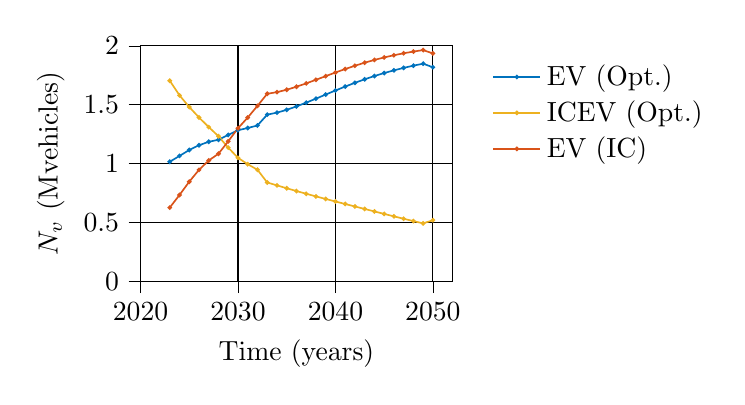
\begin{tikzpicture}

% This file was created with tikzplotlib v0.10.1.
\definecolor{mycolor1}{rgb}{0.00000,0.44700,0.74100}%
\definecolor{mycolor2}{rgb}{0.85000,0.32500,0.09800}%
\definecolor{mycolor3}{rgb}{0.92900,0.69400,0.12500}%
\definecolor{mycolor4}{rgb}{0.49400,0.18400,0.55600}%

\begin{axis}[
/pgf/number format/1000 sep={},
width=4.521in,
height=3.566in,
at={(0.758in,0.481in)},
scale=0.4,
legend cell align={left},
legend style={
  fill opacity=0,
  draw opacity=1,
  text opacity=1,
  at={(1.1,0.97)},
  anchor=north west,
  draw=none
},
tick align=outside,
tick pos=left,
x grid style={black},
xlabel={Time (years)},
xmajorgrids,
xmin=2020, xmax=2052,
xtick style={color=black},
y grid style={black},
ylabel={$N_v$ (Mvehicles)},
ymajorgrids,
ymin=0, ymax=2,
ytick style={color=black}
]

\addplot [semithick, mycolor1, mark=*, mark size=.5, mark options={solid}]
table {%
% 2023 0.487915373797759
% 2024 0.580141012593455
% 2025 0.679180799456102
% 2026 0.769264179665754
% 2027 0.840891102769377
% 2028 0.892522139934729
% 2029 0.990529707390979
% 2030 1.10020004407093
% 2031 1.2395041085345
% 2032 1.36711132895574
% 2033 1.47896111269303
% 2034 1.5456231824534
% 2035 1.60770833879882
% 2036 1.6647654940671
% 2037 1.72159357770266
% 2038 1.76776705466067
% 2039 1.80829894181361
% 2040 1.84303096980403
% 2041 1.87622481968927
% 2042 1.89885337850183
% 2043 1.91973824478972
% 2044 1.93044536336938
% 2045 1.93960978480569
% 2046 1.94024147761993
% 2047 1.94339389121958
% 2048 1.94097296006844
% 2049 1.94159159037137
% 2050 1.93047554787411

2023 1.01517927904732
2024 1.06467183121248
2025 1.11519865799253
2026 1.1557135713313
2027 1.18471142318081
2028 1.20203520853632
2029 1.24291730044253
2030 1.2831198606974
2031 1.30174932808686
2032 1.32345233175703
2033 1.4154064917187
2034 1.43233137434477
2035 1.45625342319946
2036 1.48512134800008
2037 1.51724599382448
2038 1.55123387348811
2039 1.58592484972935
2040 1.62039571128848
2041 1.65384700243842
2042 1.68571720856938
2043 1.71560340930812
2044 1.74330315840776
2045 1.76868313381304
2046 1.79172890567911
2047 1.81252999716017
2048 1.83127810029943
2049 1.84824414494137
2050 1.81754743365601
};
\addlegendentry{EV (Opt.)}

\addplot [semithick, mycolor3, mark=*, mark size=.5, mark options={solid}]
table {%
% 2023 2.2304224637159
% 2024 2.06374629998324
% 2025 1.91634389165265
% 2026 1.77774097825141
% 2027 1.65349589829886
% 2028 1.54141437851123
% 2029 1.3871751314301
% 2030 1.23160244506136
% 2031 1.05666366746498
% 2032 0.903507518839891
% 2033 0.775581675439543
% 2034 0.701289006953526
% 2035 0.638682349272067
% 2036 0.586685980620093
% 2037 0.538957343773556
% 2038 0.504447274866104
% 2039 0.476803840092802
% 2040 0.455087518339097
% 2041 0.434071193985355
% 2042 0.422135366361461
% 2043 0.410022138491716
% 2044 0.405993825248417
% 2045 0.401324560567948
% 2046 0.403059158202547
% 2047 0.40031975309795
% 2048 0.401490235463273
% 2049 0.398328908458847
% 2050 0.405951489476035

2023 1.70315855846634
2024 1.57921548136421
2025 1.48032603311622
2026 1.39129158658586
2027 1.30967557788741
2028 1.23190130990965
2029 1.13478753837855
2030 1.04868262843489
2031 0.994418447912606
2032 0.947166516038613
2033 0.839136296413857
2034 0.814580815062154
2035 0.790137264871424
2036 0.766330126687121
2037 0.743304927651748
2038 0.720980456038655
2039 0.699177932177081
2040 0.677722776854636
2041 0.656449011236205
2042 0.635271536293914
2043 0.614156973973312
2044 0.593136030210035
2045 0.572251211560599
2046 0.551571730143368
2047 0.531183647157362
2048 0.511185095232278
2049 0.491676353888846
2050 0.518879603694141

};
\addlegendentry{ICEV (Opt.)}

\addplot [semithick, mycolor2, mark=*, mark size=.5, mark options={solid}]
table {%
2023 0.62580652378235
2024 0.733020415911391
2025 0.845749378103449
2026 0.946376442791526
2027 1.02582653254529
2028 1.08335491076081
2029 1.18873546521644
2030 1.29958796087198
2031 1.3905438807877
2032 1.48972475109184
2033 1.59262823621004
2034 1.6063756014762
2035 1.62690518534374
2036 1.65228975273203
2037 1.68088941469848
2038 1.71131195105727
2039 1.74237556984323
2040 1.77313400618992
2041 1.80276439570704
2042 1.83069824918656
2043 1.85653620962151
2044 1.88009327621429
2045 1.90125579787058
2046 1.92003479917163
2047 1.93654886404368
2048 1.9510212746768
2049 1.96375474999276
2050 1.9357186557451
};
\addlegendentry{EV (IC)}

\end{axis}

\end{tikzpicture}

       % \caption{}
       % \label{fig:Nv}
    \end{subfigure}
    \hspace{1cm}
    \begin{subfigure}[t]{\columnwidth}
        \centering
        % \pgfplotsset{ylabel shift = -.5em} % Adjusts the ylabel 
        % This file was created with tikzplotlib v0.10.1.
\definecolor{mycolor1}{rgb}{0.00000,0.44700,0.74100}%
\definecolor{mycolor2}{rgb}{0.85000,0.32500,0.09800}%
\definecolor{mycolor3}{rgb}{0.92900,0.69400,0.12500}%
\definecolor{mycolor4}{rgb}{0.49400,0.18400,0.55600}%

\begin{tikzpicture}

\definecolor{darkgray176}{RGB}{176,176,176}
\definecolor{lightgray204}{RGB}{204,204,204}
\definecolor{steelblue31119180}{RGB}{31,119,180}

\begin{axis}[
/pgf/number format/1000 sep={},
width=4.521in,
height=3.566in,
at={(0.758in,0.481in)},
scale=0.4,
legend cell align={left},
legend style={fill opacity=0.2, draw opacity=1, text opacity=1, draw=none,
at={(1.1,0.97)},
 anchor=north west},
tick align=outside,
tick pos=left,
x grid style={darkgray176},
xlabel={Time (years)},
xmajorgrids,
xmin=2020, xmax=2052,
xtick style={color=black},
y grid style={darkgray176},
ylabel={$S_v$ (Mvehicles)},
ymajorgrids,
ymin=0, ymax= 40,%37.2816403,
ytick style={color=black}
]
\addplot [semithick, mycolor1, mark=*, mark size=.5, mark options={solid}]
table {%
% 2022 0.276883
% 2023 0.764090962694169
% 2024 1.34310892746958
% 2025 2.02060261436294
% 2026 2.78741761556419
% 2027 3.62453178628265
% 2028 4.51102768609597
% 2029 5.48964560797065
% 2030 6.56661640406288
% 2031 7.76542042219597
% 2032 9.0677017602779
% 2033 10.4508846387643
% 2034 11.863190841766
% 2035 13.2935907190025
% 2036 14.7306493348113
% 2037 16.1676572314484
% 2038 17.5875008002173
% 2039 18.9783494297071
% 2040 20.3289340104888
% 2041 21.6332027477994
% 2042 22.8770985100598
% 2043 24.0564061747522
% 2044 25.1595199496494
% 2045 26.1845066744693
% 2046 27.1234338863994
% 2047 27.9803184333338
% 2048 28.7519162793243
% 2049 29.4443266083617
% 2050 30.0495276503

2022 0.276883
2023 1.29135486794373
2024 2.35490365133818
2025 3.46841519676797
2026 4.62167958963476
2027 5.80261408076466
2028 6.99862304917957
2029 8.22592828929042
2030 9.47330873035929
2031 10.7086343782447
2032 11.9247898406515
2033 13.182615207678
2034 14.3988247635827
2035 15.5733888339143
2036 16.7055196332013
2037 17.7942620455312
2038 18.8388496202931
2039 19.8383784348856
2040 20.7922292117582
2041 21.7002550093439
2042 22.562786288021
2043 23.3805539520607
2044 24.154661719457
2045 24.8864443852979
2046 25.5774007359189
2047 26.2291441522406
2048 26.8433829691061
2049 27.4219125398571
2050 27.9204094245999
};
\addlegendentry{EV (Opt.)}

% \addplot [semithick, mycolor2,  mark=*, mark size=.5, mark options={solid}]
% table {%
% 2022 0.276883
% 2023 0.996574760046214
% 2024 1.80861697235832
% 2025 2.7140082700907
% 2026 3.69586194261096
% 2027 4.72459044250431
% 2028 5.77248866927143
% 2029 6.92516200306705
% 2030 8.19041597955684
% 2031 9.53322190016517
% 2032 10.9658757202515
% 2033 12.4891892437799
% 2034 13.8949473996703
% 2035 15.2006852101302
% 2036 16.4195543076723
% 2037 17.5616021476254
% 2038 18.6347236466039
% 2039 19.6453066723808
% 2040 20.6564385012813
% 2041 21.6718123764221
% 2042 22.6842607706148
% 2043 23.6869004819276
% 2044 24.6733091849939
% 2045 25.6376590336468
% 2046 26.5748097122809
% 2047 27.4803596854156
% 2048 28.3506617811441
% 2049 29.1828085214691
% 2050 29.9628533020153
% };
% \addlegendentry{EV (M1)}
\addplot [semithick, mycolor3, mark=*, mark size=.5, mark options={solid}]
table {%
% 2022 35.519509
% 2023 35.3097968360154
% 2024 34.97352716277
% 2025 34.531333879387
% 2026 33.9923713936746
% 2027 33.3756618504272
% 2028 32.7021226900652
% 2029 31.9290136196203
% 2030 31.0501037869346
% 2031 30.041912844192
% 2032 28.9227966934791
% 2033 27.7153311143439
% 2034 26.4712943226718
% 2035 25.2017159687454
% 2036 23.918030988227
% 2037 22.6269488388605
% 2038 21.3455831293426
% 2039 20.0857644710823
% 2040 18.8587619735122
% 2041 17.6706274313918
% 2042 16.5354179762965
% 2043 15.4573487307549
% 2044 14.4480254869889
% 2045 13.5093814052786
% 2046 12.6493489484385
% 2047 11.8639112685745
% 2048 11.1563124016346
% 2049 10.5204531636282
% 2050 9.96435532469948

2022 35.519509
2023 34.7825329307659
2024 33.9617324389014
2025 33.083521296982
2026 32.158109419604
2027 31.1975795559451
2028 30.2145273269816
2029 29.1927309383006
2030 28.1434114606382
2031 27.0986988881433
2032 26.0657086131055
2033 24.9836005454302
2034 23.9356604008552
2035 22.9219178538336
2036 21.943160689837
2037 21.0003440247777
2038 20.0942343092667
2039 19.2257354659038
2040 18.3954667722428
2041 17.6035751698473
2042 16.8497301983353
2043 16.1332009534464
2044 15.4528837171812
2045 14.80744369445
2046 14.195382098919
2047 13.6150855496677
2048 13.0648457118528
2049 12.5428672321329
2050 12.0934735503995
};
\addlegendentry{ICEV (Opt.)}
\addplot [color=mycolor2, mark=*, mark options={solid, mycolor2}, mark size=.5]
  table[row sep=crcr]{%
2022	0.276883\\
2023	0.90198211267876\\
2024	1.63387948077211\\
2025	2.47794174631282\\
2026	3.42186901063984\\
2027	4.44391861113421\\
2028	5.52124728177362\\
2029	6.69710325793011\\
2030	7.97000666968697\\
2031	9.31230240582858\\
2032	10.7239404782539\\
2033	12.2002755811868\\
2034	13.6441437964197\\
2035	15.0546221112408\\
2036	16.4291370157325\\
2037	17.7640184007189\\
2038	19.0548684113387\\
2039	20.2967919404005\\
2040	21.4852832249128\\
2041	22.6165959604329\\
2042	23.6878800947605\\
2043	24.6972043125328\\
2044	25.6436017441817\\
2045	26.5269593070818\\
2046	27.3479553979408\\
2047	28.1079858433601\\
2048	28.8090953418799\\
2049	29.4539002713503\\
2050	30.0061194771407\\
};
\addlegendentry{EV (IC)}

\end{axis}

\end{tikzpicture}

        %\caption{}
        %\label{fig:stock}
    \end{subfigure}
    % \hspace{1cm}
    \caption{Vehicle Sales (top) and Vehicle Stock (bottom) }\label{fig:salesStock}
\end{figure}


\subsection{Results}
%%%%%%%%%%%%%%%%%%%%%%%%%%%%%%%%%%%%%%%%%%%%%%%

The emissions, and vehicle sales and stock curves, for IC and optimal scenario, are shown in Fig.~\ref{fig:opt}~(right), and Fig.~\ref{fig:salesStock}, respectively. Clearly, in both scenarios, the ICEV stock ($v=1$) decreases while the EV stock ($v=2$) increases with time, both exhibiting an S-shaped curve suggesting variable rate. The curve of CO$_2$ emissions, Fig.~\ref{fig:opt}~(right), is proportional to that of $S_1$ and decreases by more than three times with respect to 2022. The IC scenario forecasts 12.3~Mt of CO$_2$ in 2050. Correspondingly, $\overline{E}$ is set to this value. 

The incentive law shown in  Fig.~\ref{fig:opt}~(left) exhibits a very variable behavior, being null until a certain year, to rise up by the end of the period. Intuitively, such a behavior is optimal, within the assumptions of the model, in that it incentivises late adopters and encourages EV purchase during a period when ICE performance is improving. 
and further reduce the emissions while minimizing the total budget. This effect is visible in the curves of EV sales and stock (Fig.~\ref{fig:salesStock}) and emissions (Fig.~\ref{fig:opt}~(right)). Compared to the IC law,  EV sales are lower in the initial years and begin to increase around midpoint. Consequently, the optimal emission curve decreases gradually in the early years and exhibits a sharper decrease towards the end. The final CO$_2$ emission for both scenarios are equal as the  constraint is defined only at $T$. However, the cumulative CO$_2$ emissions of the optimal scenario is higher than the IC scenario. To address this, an integral constraint on emissions can be defined in future work.  
Regarding the EV stock, it increases gradually early-on but shows a sharper increase towards the end as result of the optimal incentive. 

Overall, we obtain a total expenditure $I(T)= 196.2$ G\euro, that is, around 30\% reduction with respect to the IC reference scenario, see Table~\ref{tab:res}.    

\subsection{Alternative scenarios}\label{sec:alter}
%%%%%%%%%%%%%%%%%%%%%%%%%%%%%%%%%%%

In addition to the optimal and IC scenarios, we analyze three different policies, namely,
\begin{itemize}
    \item No incentive (I0), $u(t) \equiv 0$ 
    %\item Constant incentive (IC), $u(t) \equiv 5$ k\euro  
    \item Incentive covering the whole EV price (IP), $u(t) = C_2^P(t)$
    \item Ban of ICEV sales from $t_0$ (BI), $N_{2}(t) = N(t)$
\end{itemize}
%
The corresponding curves of CO$_2$ emissions and EV stock are shown in Fig.~\ref{fig:refs}. Clearly, the more stringent the policy, the faster increase of EV stock is observed, together with a decrease in yearly emissions. With the BI, the ICEV stock virtually empties by 2050 and consequently the CO$_2$ emissions vanish by that target year. The $E(T)$ and $I(T)$ values for the different policy scenarios are given in Table~\ref{tab:res}.

\begin{figure}[h!] 
    \centering
    \begin{subfigure}[t]{\columnwidth}
        \centering
        %\pgfplotsset{ylabel shift = -.5em} % Adjusts the ylabel 
        % This file was created by matlab2tikz.
%
%The latest updates can be retrieved from
%  http://www.mathworks.com/matlabcentral/fileexchange/22022-matlab2tikz-matlab2tikz
%where you can also make suggestions and rate matlab2tikz.
%
\definecolor{mycolor1}{rgb}{0.00000,0.44700,0.74100}%
\definecolor{mycolor2}{rgb}{0.85000,0.32500,0.09800}%
\definecolor{mycolor3}{rgb}{0.92900,0.69400,0.12500}%
\definecolor{mycolor4}{rgb}{0.49400,0.18400,0.55600}%
%
\begin{tikzpicture}

\begin{axis}[%
/pgf/number format/1000 sep={},
width=4.521in,
height=3.566in,
at={(0.758in,0.481in)},
scale =.4,
xmin=2020,
xmax=2052,
xlabel style={font=\color{white!15!black}},
xlabel={Time (years)},
ymin=-2,
ymax=65,
ylabel style={font=\color{white!15!black}},
ylabel={$E$ (Mt)},
axis background/.style={fill=white},
xmajorgrids,
ymajorgrids,
legend style={at={(1.1,.97)}, anchor=north west, legend cell align=left, align=left, draw=none, fill opacity=0.8}
]
\addplot [color=mycolor1, mark=*, mark options={solid, mycolor1}, mark size=.5]
  table[row sep=crcr]{%
2022	62.0973386775\\
2023	60.3772061729652\\
2024	58.5655250320406\\
2025	56.6930285796768\\
2026	54.7698219810999\\
2027	52.8296600717508\\
2028	50.8844656595381\\
2029	48.8888122329172\\
2030	46.840855906383\\
2031	44.760913732486\\
2032	42.6405497339573\\
2033	40.468819463666\\
2034	38.375787677183\\
2035	36.3531099403197\\
2036	34.3985618075106\\
2037	32.532486521514\\
2038	30.7057871997411\\
2039	28.9683729218248\\
2040	27.3185351239776\\
2041	25.7558635321482\\
2042	24.2646197819138\\
2043	22.8586192926125\\
2044	21.5378434203587\\
2045	20.3026815623895\\
2046	19.1482585401559\\
2047	18.0783267996862\\
2048	17.0778073973195\\
2049	16.1506154509676\\
2050	15.3215713193231\\
};
\addlegendentry{I0}

\addplot [color=mycolor2, mark=*, mark options={solid, mycolor2}, mark size=.5]
  table[row sep=crcr]{%
2022	62.0973386775\\
2023	60.1836066576528\\
2024	58.1593466433033\\
2025	56.0574852427096\\
2026	53.8927857845427\\
2027	51.7029605179969\\
2028	49.5027172631407\\
2029	47.2461952797078\\
2030	44.9385068147861\\
2031	42.6121506008471\\
2032	40.2665216203798\\
2033	37.8983092627524\\
2034	35.6270367242917\\
2035	33.446161445072\\
2036	31.3547818773782\\
2037	29.3718667035712\\
2038	27.4509062460178\\
2039	25.6416200529808\\
2040	23.9416930704035\\
2041	22.347770786495\\
2042	20.8449561356326\\
2043	19.4437224049606\\
2044	18.1443956814805\\
2045	16.9438462199866\\
2046	15.8372562880573\\
2047	14.8249199677192\\
2048	13.8917475730213\\
2049	13.0384358223612\\
2050	12.2822247684378\\
};
\addlegendentry{IC}

\addplot [color=mycolor3, mark=*, mark options={solid, mycolor3}, mark size=.5]
  table[row sep=crcr]{%
2022	62.0973386775\\
2023	58.7223564746349\\
2024	55.3012184625432\\
2025	51.8747599714611\\
2026	48.4665169250132\\
2027	45.1128889718546\\
2028	41.824636303344\\
2029	38.588923706835\\
2030	35.4343880572894\\
2031	32.3903154323214\\
2032	29.4742336848917\\
2033	26.6935893006537\\
2034	24.1001622652403\\
2035	21.6911997086484\\
2036	19.466136748236\\
2037	17.4358212160008\\
2038	15.5542730620576\\
2039	13.8638097030724\\
2040	12.3533559832307\\
2041	11.0053001882722\\
2042	9.79984113216183\\
2043	8.73318347113825\\
2044	7.80070907455796\\
2045	6.98622610477781\\
2046	6.28097052761465\\
2047	5.67424371690844\\
2048	5.14866273304823\\
2049	4.69634039844939\\
2050	4.30014740913832\\
};
\addlegendentry{IP}

\addplot [color=mycolor4, mark=*, mark options={solid, mycolor4}, mark size=.5]
  table[row sep=crcr]{%
2022	62.0973386775\\
2023	57.245692693174\\
2024	52.5643722590114\\
2025	48.0530702524094\\
2026	43.7059135411688\\
2027	39.5335316421169\\
2028	35.5282360685896\\
2029	31.7193255315308\\
2030	28.1293588279806\\
2031	24.7717666282476\\
2032	21.6599659491601\\
2033	18.7950313188431\\
2034	16.1808434546874\\
2035	13.8145286760166\\
2036	11.6928169436272\\
2037	9.8194005597368\\
2038	8.14413720479249\\
2039	6.70151432013578\\
2040	5.47205851709268\\
2041	4.4276239453184\\
2042	3.54232659076817\\
2043	2.8027270151109\\
2044	2.19929010791141\\
2045	1.7079486749557\\
2046	1.31683557132408\\
2047	1.00957371169903\\
2048	0.767686614436828\\
2049	0.579754571869599\\
2050	0.419126668371727\\
};
\addlegendentry{BI}

\end{axis}


\end{tikzpicture}%
        %\caption{}
    \end{subfigure}
    \hspace{1cm}
    \begin{subfigure}[t]{\columnwidth}
        \centering
        %\pgfplotsset{ylabel shift = -.5em} % Adjusts the ylabel 
        % This file was created by matlab2tikz.
%
%The latest updates can be retrieved from
%  http://www.mathworks.com/matlabcentral/fileexchange/22022-matlab2tikz-matlab2tikz
%where you can also make suggestions and rate matlab2tikz.
%
\definecolor{mycolor1}{rgb}{0.00000,0.44700,0.74100}%
\definecolor{mycolor2}{rgb}{0.85000,0.32500,0.09800}%
\definecolor{mycolor3}{rgb}{0.92900,0.69400,0.12500}%
\definecolor{mycolor4}{rgb}{0.49400,0.18400,0.55600}%
%
\begin{tikzpicture}

\begin{axis}[%
/pgf/number format/1000 sep={},
width=4.521in,
height=3.566in,
at={(0.758in,0.481in)},
scale =.4,
xmin=2020,
xmax=2052,
xlabel style={font=\color{white!15!black}},
xlabel={Time (years)},
ymin=-2,
ymax=42,
ylabel style={font=\color{white!15!black}},
ylabel={$S_2$ (Mvehicles)},
axis background/.style={fill=white},
xmajorgrids,
ymajorgrids,
legend style={at={(1.1,0.97)}, 
anchor=north west, 
legend cell align=left, 
align=left, 
draw=none, 
fill opacity=0.8}
]
\addplot [color=mycolor1, mark=*, mark options={solid, mycolor1},, mark size=.5]
  table[row sep=crcr]{%
2022	0.276883\\
2023	0.764090720006111\\
2024	1.34310863939405\\
2025	2.02060231508006\\
2026	2.78741710446031\\
2027	3.62453088480891\\
2028	4.51102615279705\\
2029	5.48964332250078\\
2030	6.56396393107977\\
2031	7.71554823951511\\
2032	8.95042866333868\\
2033	10.2700569397255\\
2034	11.5690713659481\\
2035	12.848016378594\\
2036	14.105449518351\\
2037	15.3384870919928\\
2038	16.5431582723137\\
2039	17.7146193606683\\
2040	18.8481157382805\\
2041	19.9394168507441\\
2042	20.984976630418\\
2043	21.9819912260398\\
2044	22.9284789709706\\
2045	23.8232150217884\\
2046	24.6657077362019\\
2047	25.4561605230879\\
2048	26.1954340401284\\
2049	26.8849951828921\\
2050	27.4806489361322\\
};
\addlegendentry{I0}

\addplot [color=mycolor2, mark=*, mark options={solid, mycolor2}, mark size=.5]
  table[row sep=crcr]{%
2022	0.276883\\
2023	0.90198211267876\\
2024	1.63387948077211\\
2025	2.47794174631282\\
2026	3.42186901063984\\
2027	4.44391861113421\\
2028	5.52124728177362\\
2029	6.69710325793011\\
2030	7.97000666968697\\
2031	9.31230240582858\\
2032	10.7239404782539\\
2033	12.2002755811868\\
2034	13.6441437964197\\
2035	15.0546221112408\\
2036	16.4291370157325\\
2037	17.7640184007189\\
2038	19.0548684113387\\
2039	20.2967919404005\\
2040	21.4852832249128\\
2041	22.6165959604329\\
2042	23.6878800947605\\
2043	24.6972043125328\\
2044	25.6436017441817\\
2045	26.5269593070818\\
2046	27.3479553979408\\
2047	28.1079858433601\\
2048	28.8090953418799\\
2049	29.4539002713503\\
2050	30.0061194771407\\
};
\addlegendentry{IC}

\addplot [color=mycolor3, mark=*, mark options={solid, mycolor3}, mark size=.5]
  table[row sep=crcr]{%
2022	0.276883\\
2023	1.94275859630977\\
2024	3.67924280204581\\
2025	5.48524921463686\\
2026	7.34119964602009\\
2027	9.22532531067205\\
2028	11.1167276166683\\
2029	13.033159738462\\
2030	14.9544919695955\\
2031	16.8546197236402\\
2032	18.7185467046846\\
2033	20.532052113359\\
2034	22.2505828732729\\
2035	23.8698426699347\\
2036	25.3864047645767\\
2037	26.7979073407248\\
2038	28.1031481145103\\
2039	29.3020929008776\\
2040	30.396113327194\\
2041	31.3878861499674\\
2042	32.2812878614017\\
2043	33.0811692224301\\
2044	33.7931850646948\\
2045	34.4234771791942\\
2046	34.9784588380751\\
2047	35.4646313774455\\
2048	35.8884526528261\\
2049	36.2562371792307\\
2050	36.5649091272265\\
};
\addlegendentry{IP}

\addplot [color=mycolor4, mark=*, mark options={solid, mycolor4}, mark size=.5]
  table[row sep=crcr]{%
2022	0.276883\\
2023	2.99451342641007\\
2024	5.63727769116873\\
2025	8.23111526971474\\
2026	10.7756712491674\\
2027	13.2662813181847\\
2028	15.6941915965093\\
2029	18.0443318126144\\
2030	20.2998858464384\\
2031	22.4457899245698\\
2032	24.469308255942\\
2033	26.3603083848646\\
2034	28.1114522557907\\
2035	29.7182529965896\\
2036	31.1789829659319\\
2037	32.4945500232209\\
2038	33.6682873682154\\
2039	34.7056635346217\\
2040	35.613985795169\\
2041	36.4019224158842\\
2042	37.0791797602718\\
2043	37.6560781425844\\
2044	38.1432227102626\\
2045	38.5510590988991\\
2046	38.8895814344837\\
2047	39.1681168349862\\
2048	39.3952037070307\\
2049	39.5785361600049\\
2050	39.7248865118169\\
};
\addlegendentry{BI}

\end{axis}

\end{tikzpicture}%
        %\caption{}
    \end{subfigure}
    \caption{Reference Scenarios with the full model: CO$_2$ emissions (top) and EV stock (bottom) as a function of time.}\label{fig:refs}
\end{figure}

\begin{table}[h!]
    \centering
    \caption{Reference and optimal scenario}    \label{tab:res}
    \begin{tabular}{c|ccccc}
    \hline
              Output  & I0  & IC  & IP  & BI  & Optimal  \\
    \hline
       $E(T)$ (Mt) &   15.3 & 12.3 & 4.3 & 0.4 & 12.3 \\
         $I(T)$ (G\euro) & 0 & 215 & 1497 & - & 196.2 \\
         \hline
        %Refined & 12.2 &   215 & 12.2 & 196.2\\ \hline
    \end{tabular}
\end{table}



\section{Conclusions and Future Work}
%%%%%%%%%%%%%%%%%%%%%%%%%%%%%%%%%%%%%%%%%%%%%%

This study represents a first attempt to build a backcasting methodology to identify the optimal policy roadmaps in transport systems. 
The analysis focussed on a passenger car fleet subsystem, describing its evolution and associated emissions, with the monetary incentive to an EV purchase as the control input. The optimal incentive trajectory was derived by formulating an optimal control problem with the objective to minimize the state's budget while reaching a desired CO$_2$ target. A quantitative case study applied to Metropolitan France was performed to illustrate the backcasting approach. 

Further research can improve the backcasting paradigm in several ways. Refinements to the fleet model could include regional disaggregation within Metropolitan France, additional vehicle types (e.g., gasoline, diesel, hybrid) and transport modes (e.g., bikes, rail), and modeling second-hand vehicle exchanges. Mileage assumptions could be refined by accounting for variation by vehicle type and user profile, using zone-specific data (e.g., urban, rural) as in (\cite{ITF}). The survival rate, currently based only on natural obsolescence, could also incorporate factors like Low Emission Zones (LEZ), which can accelerate vehicle turnover. Additionally, the zonal choice in a LEZ implementation could be optimized.  Finally, to capture the changes in operating costs and vehicle ownership, the demand for passenger cars, treated here as exogenous, could be replaced with a demand model predicting vkm by mode and zone.

% Further research can improve the presented backcasting paradigm in several different directions. Firstly, refinements to the fleet model can include disaggregating Metropolitan France into smaller zones, including more vehicle types (e.g., gasoline, diesel, hybrid) and transportation modes (e.g., bike, powered-two-wheelers, rail), modelling second-hand vehicle movement between private and professional ownerships, and distinction between registered and circulating fleet.
% %
% Similarly, mileage is likely not constant for all users and vehicles in a given zone. A differentiation of the latter by veh-type, using typical usage profiles by zone or zone category (e.g., urban, peri-urban, rural) as done in (\cite{ITF} could therefore be considered in a future version of the model.
% %
% The current survival rate implementation considers only natural vehicle obsolescence. Other factors such as Low Emission Zones (LEZ) can decrease the survival rata. Furthermore, the decision to set up a LEZ for a certain zone can be optimized. 
% %
% Secondly, the demand for passenger cars has been considered as exogenous in this work. To capture the effects of operating cost and ownership changes, a demand model that predicts the vkm by zone and mode is thus necessary. 

% However, a change in operating costs and in vehicle ownership will likely have an effect on the share of this transportation mode with respect to others (public transport, walking, etc.) To capture this effects, a demand model that predicts the vkm by zone and mode is thus necessary.
% Similarly, mileage is likely not constant for all users and vehicles in a given zone. A differentiation of the latter by veh-type, using typical usage profiles by zone or zone category (e.g., urban, peri-urban, rural) as done in (\cite{ITF} could therefore be considered in a future version of the model.
% Some types of vehicles are not only scrapped because of their natural obsolescence, but also for other reasons that are linked to decisions that could be optimized. For example, the set up of low emission zones in some urban areas could bring to the riddance of the vehicle types forbidden by a higher rate that the natural survival rate. The decision to set up a LEZ by zone could be then optimized with the constraint of minimize the forced number of vehicle dumped. 

% The adoption coefficient can be also made endogenous to capture the influence of variable prices and operational costs, which is not the case in the present model. 
% %
% An anticipation of future bans could be treated similarly to a negative-adoption coefficient that decreases the utility function for ICEVs without strictly forbidding their sales.

% These extensions of the backcasting approach would require further refinements to the fleet model itself. First off, multiple zones must be considered since setting a LEZ is a typically local policy. Also, multiple vehicle types (e.g., gasoline, diesel, hybrid) must be considered, since LEZ regulations distinguish between them. 
% The in-use (or circulating) fleet could be considered when evaluating the emissions, instead of the registered fleet. 

%%%%%%%%%%%%%%%%%%%%%%%%%%%%%%%%%%%%%%
\section*{Acknowledgments}
This research benefited from state aid managed by the \textit{Agence Nationale de la Recherche (ANR)}, under France 2030, within the project FORBAC bearing the reference ANR-23-PEMO-0002. The authors would like to acknowledge the useful discussions with Dr. Benoit Cheze (IFPEN) and the partners of the FORBAC project. 
%A CC-BY public copyright license has been applied by the authors to the present document and will be applied to all subsequent versions up to the Author Accepted Manuscript arising from this submission, in accordance with the grant’s open access conditions.

%%%%%%%%%%%%%%%%%%%%%%%%%%%%%%%%%%%%%%%%%%%%%
\bibliography{parc_aac} 


% \begin{thebibliography}{99}

% \bibitem{GreenDeal} European Commission (2021), ``European Green Deal: Commission proposes transformation of EU economy and society to meet climate ambitions", Press Release, available at \url{https://ec.europa.eu/commission/presscorner/}.

% \bibitem{EPA} Environmental Protection Agency (2023), ``Multi-Pollutant Emissions Standards for Model Years 2027 and Later Light-Duty and Medium-Duty Vehicles", available at \url{https://www.epa.gov}.

% \bibitem{TREMOVE} De Ceuster G et al. (2004), TREMOVE 2.2 Model and Baseline Description, 
% Report for European Commission, available at \url{www.asser.nl}.

% \bibitem{High-Tool} Van Grol R et al. (2016), ``Elasticities and Equations of the HIGH-TOOL
% Model (Final Version)", HIGH-TOOL Deliverable D4.3, project cofunded by the European Commission under the 7th Framework Programme, Karlsruhe.

% \bibitem{ITF} International Transport Forum (2019), ``Understanding Consumer Vehicle Choice: A New Car Fleet Model for France", International Transport Forum Policy Papers No. 72, OECD Publishing, Paris.

% \bibitem{ADEME} Bouter A et al. (2022), ``Etude énergétique, économique et environnementale du transport routier à horizon 2040 (E4T 2040), IFPEN-ADEME, available at \url{https:\\librairie.ademe.fr}.

% \bibitem{train} Train KE (2003), ``Discrete Choice Methods with Simulation", Cambridge Univ. Press, Cambridge, 2nd ed.

% \bibitem{benakiva} Ben-Akiva L, Lerman SR (2000), ``Discrete Choice Analysis", MIT press, Cambridge MA.

% \bibitem{thorne} Thorne R, Aguilar Lopez F, Figenbaum E, Fridstrøm L, Müller DB (2021), ``Estimating stocks and flows of electric passenger vehicle batteries in the Norwegian fleet from 2011 to 2030", Journal of Industrial Ecology, 25(6):1377--1706.

% \bibitem{sato} Kenta Sato FE, Nakata T (2020), ``Recoverability Analysis of Critical Materials from Electric Vehicle Lithium-Ion Batteries through a Dynamic Fleet-Based Approach for Japan", Sustainability, 12(1), 147.

% \bibitem{woody} Woody M., Keoleian GA, Vaishnav P (2023), ``Decarbonization potential of electrifying 50\% of U.S. light-duty vehicle sales by 2030". Nat Commun 14, 7077.

% \bibitem{Bass} Bass FM (1969), ``A New-Product Growth Model for Consumer Durables", Management Science, 15, 1,215-227.

% \bibitem{macmanus} McManus W, Senter R (2009), ``Market Models for Predicting PHEV Adoption and Diffusion", U.S. Department of Energy, Final Report, available at \url{https://deepblue.lib.umich.edu/}.

% \bibitem{sterman} Struben J, Sterman J (2008), ``Transition Challenges for ALternative Fuel Vehicle and Transportation Systems", Environment and Planning B, 35(6):1070--1097.


% \end{thebibliography}

%%%%%%%%%%%%%%%%%%%%%%%%%%%%%%%%%%%%%%%%%%%%%%

% \appendix

% \section{Parameters and Exogenous Variables}

% \begin{table}[h!]
%     \centering
%     \caption{List of parameters for Metropolitan France.}   
%     \label{tab:logit}
%     \begin{tabular}{ccc}
%         Attributes & ICEV & EV \\ \hline
%         Purchase Cost ($p^P$) & -0.3 & -0.3\\
%         Operating Cost ($p^O$) & -0.15 & -0.15\\
%         Infrastructure Cost ($p^I$) & - & -0.3\\
%         $\mu$ & \multicolumn{2}{c}{6.75} \\ \hline
%     \end{tabular}
%     \label{tab:param}
% \end{table}

% \begin{table}[!ht]
%     \centering
%     \caption{Initial stocks, emission factor, and survival rate by veh-type and veh-age} \label{tab:instock}
%     \begin{tabular}{ccccc} \hline Age & \multicolumn{2}{c}{{Initial stock}} & Emission factor & Survival rate \\ $a$ & $S_1(t_0)$ & $S_2(t_0)$ & $\epsilon_{1,0}(t)$ & $\eta_a$ \\ \hline
%         0  & 850729 & 107751 &   105.8  & N.A. \\ 
%         1  & 1208829 & 77284 &    107  & 1.0  \\ 
%         2  & 1911867 & 25646 &    108  & 1.0  \\ 
%         3  & 2001224 & 18161 &    115  & 0.999  \\ 
%         4  & 1922874 & 14580 &    114  & 0.944  \\ 
%         5  & 1915687 & 12701 &    113  & 1.011  \\ 
%         6  & 1815720 & 9332 &    112  & 0.993  \\ 
%         7  & 1715103 & 4653 &    113  & 0.996  \\ 
%         8  & 1704027 & 3695 &    116  & 0.981  \\ 
%         9  & 1773074 & 2013 &    119  & 0.983  \\ 
%         10  & 1992409 & 716 &    124  & 0.975  \\ 
%         11  & 1984333 & 61 &    128  & 0.978  \\ 
%         12  & 1941219 & 64 &    130  & 0.964  \\ 
%         13  & 1734257 & 23 &    133  & 0.962  \\ 
%         14  & 1656124 & 18 &    140  & 0.945  \\ 
%         15  & 1461471 & 11 &    151  & 0.941  \\ 
%         16  & 1282236 & 7 &    151  & 0.919  \\ 
%         17  & 1116991 & 9 &    154  & 0.914  \\ 
%         18  & 970820 & 5 &    156  & 0.895  \\ 
%         19  & 874548 & 25 &    157  & 0.892  \\ 
%         20  & 762675 & 20 &    158  & 0.871  \\ 
%         21  & 632719 & 15 &    159  & 0.875  \\ 
%         22  & 511403 & 32 &    162  & 0.858  \\ 
%         23  & 353184 & 27 &    166  & 0.859  \\ 
%         24  & 230132 & 10 &    171  & 0.845  \\ 
%         25  & 199309 & 4 &    175  & 0.785  \\ 
%         26  & 199309 & 4 &    175  & N.A.  \\ 
%         27  & 199309 & 4 &    176  & N.A.  \\ 
%         28  & 199309 & 4 &    176  & N.A.  \\ 
%         29  & 199309 & 4 &    176  & N.A.  \\ 
%         30  & 199309 & 4 &    176 & N.A.  \\ 
%         \hline
%     \end{tabular}
% \end{table}

% \begin{table}[h!] 
% \centering
% \caption{Costs by type, veh-type, and year.} \label{tab:costs}
% \begin{tabular}{ccccccc}
% \hline
% {Year} & \multicolumn{2}{c}{{BEV({\euro})}} & \multicolumn{2}{c}{{Thermal({\euro})}} & \multicolumn{2}{c}{{Average({\euro})}} \\
% & $C_2^P(t)$ & $C_2^O(t)$ & $C_1^P(t)$ & $C_1^O(t)$ & $\overline{C}^P(t)$ & $\overline{C}^O(t)$ \\
% \hline
% 2020 & 40000 & 800.0 & 27500 & 550 & 33750 & 675.0 \\
% 2021 & 33220 & 664.4 & 27650 & 553 & 30435 & 608.7 \\
% 2022 & 32440 & 648.8 & 27800 & 556 & 30120 & 602.4 \\
% 2023 & 31660 & 633.2 & 27950 & 559 & 29805 & 596.1 \\
% 2024 & 30880 & 617.6 & 28100 & 562 & 29490 & 589.8 \\
% 2025 & 30100 & 602.0 & 28250 & 565 & 29175 & 583.5 \\
% 2026 & 29320 & 586.4 & 28400 & 568 & 28860 & 577.2 \\
% 2027 & 28540 & 570.8 & 28550 & 571 & 28545 & 570.9 \\
% 2028 & 27760 & 555.2 & 28700 & 574 & 28230 & 564.6 \\
% 2029 & 26980 & 539.6 & 28850 & 577 & 27915 & 558.3 \\
% 2030 & 26200 & 524.0 & 29000 & 580 & 27600 & 552.0 \\
% 2031 & 26090 & 521.8 & 29450 & 589 & 27770 & 555.4 \\
% 2032 & 25980 & 519.6 & 29900 & 598 & 27940 & 558.8 \\
% 2033 & 25870 & 517.4 & 30350 & 607 & 28110 & 562.2 \\
% 2034 & 25760 & 515.2 & 30800 & 616 & 28280 & 565.6 \\
% 2035 & 25650 & 513.0 & 31250 & 625 & 28450 & 569.0 \\
% 2036 & 25540 & 510.8 & 31700 & 634 & 28620 & 572.4 \\
% 2037 & 25430 & 508.6 & 32150 & 643 & 28790 & 575.8 \\
% 2038 & 25320 & 506.4 & 32600 & 652 & 28960 & 579.2 \\
% 2039 & 25210 & 504.2 & 33050 & 661 & 29130 & 582.6 \\
% 2040 & 25100 & 502.0 & 33500 & 670 & 29300 & 586.0 \\
% 2041 & 24990 & 499.8 & 33950 & 679 & 29470 & 589.4 \\
% 2042 & 24880 & 497.6 & 34400 & 688 & 29640 & 592.8 \\
% 2043 & 24770 & 495.4 & 34850 & 697 & 29810 & 596.2 \\
% 2044 & 24660 & 493.2 & 35300 & 706 & 29980 & 599.6 \\
% 2045 & 24550 & 491.0 & 35750 & 715 & 30150 & 603.0 \\
% 2046 & 24440 & 488.8 & 36200 & 724 & 30320 & 606.4 \\
% 2047 & 24330 & 486.6 & 36650 & 733 & 30490 & 609.8 \\
% 2048 & 24220 & 484.4 & 37100 & 742 & 30660 & 613.2 \\
% 2049 & 24110 & 482.2 & 37550 & 751 & 30830 & 616.6 \\
% 2050 & 25000 & 500.0 & 38000 & 760 & 31500 & 630.0 \\
% \hline
% \end{tabular}
% \end{table}

% \begin{table}[!ht] 
%     \centering
%     \caption{Coefficients of adoption and infrastructure development, by year} \label{tab:coeff}
%     \begin{tabular}{ccc}
%     \hline
%     Year & Infr. Dev. & Adoption \\
%     & $c^I_2(t)$ & $c^A_2(t)$ \\
%     \hline
%         2020  & 0.1 & 0.04 \\ 
%         2021  & 0.15 & 0.05 \\ 
%         2022  & 0.2 & 0.06 \\ 
%         2023  & 0.25 & 0.08 \\
%         2024  & 0.3 & 0.09 \\ 
%         2025  & 0.35 & 0.11 \\
%         2026  & 0.4 & 0.11 \\ 
%         2027  & 0.45 & 0.11 \\
%         2028  & 0.5 & 0.09 \\ 
%         2029  & 0.6 & 0.07 \\ 
%         2030  & 0.7 & 0.05 \\ 
%         2031  & 0.8 & 0.04 \\ 
%         2032  & 0.9 & 0.02 \\ 
%         2033  & 1 & 0.01 \\ 
%         2034  & 1 & 0.01 \\ 
%         2035  & 1 & 0.00 \\ 
%         2036  & 1 & 0.00 \\ 
%         2037  & 1 & 0.00 \\ 
%         2038  & 1 & 0.00 \\ 
%         2039  & 1 & 0.00 \\ 
%         2040  & 1 & 0.00 \\ 
%         2041  & 1 & 0.00 \\ 
%         2042  & 1 & 0.00 \\ 
%         2043  & 1 & 0.00 \\ 
%         2044  & 1 & 0.00 \\ 
%         2045  & 1 & 0.00 \\ 
%         2046  & 1 & 0.00 \\ 
%         2047  & 1 & 0.00 \\ 
%         2048  & 1 & 0.00 \\ 
%         2049  & 1 & 0.00 \\ 
%         2050  & 1 & 0.00 \\ 
%         \hline
%     \end{tabular}
% \end{table}


% \begin{table}[h!]
% \centering
% \caption{Buying Costs (\euro)}
% \begin{tabular}{cccc}
% \hline
% \textbf{Year} & \textbf{BEV} & \textbf{Thermal} & \textbf{Average} \\
% \hline
% 2020 & 40000 & 27500 & 33750 \\
% 2021 & 33220 & 27650 & 30435 \\
% 2022 & 32440 & 27800 & 30120 \\
% 2023 & 31660 & 27950 & 29805 \\
% 2024 & 30880 & 28100 & 29490 \\
% 2025 & 30100 & 28250 & 29175 \\
% 2026 & 29320 & 28400 & 28860 \\
% 2027 & 28540 & 28550 & 28545 \\
% 2028 & 27760 & 28700 & 28230 \\
% 2029 & 26980 & 28850 & 27915 \\
% 2030 & 26200 & 29000 & 27600 \\
% 2031 & 26090 & 29450 & 27770 \\
% 2032 & 25980 & 29900 & 27940 \\
% 2033 & 25870 & 30350 & 28110 \\
% 2034 & 25760 & 30800 & 28280 \\
% 2035 & 25650 & 31250 & 28450 \\
% 2036 & 25540 & 31700 & 28620 \\
% 2037 & 25430 & 32150 & 28790 \\
% 2038 & 25320 & 32600 & 28960 \\
% 2039 & 25210 & 33050 & 29130 \\
% 2040 & 25100 & 33500 & 29300 \\
% 2041 & 24990 & 33950 & 29470 \\
% 2042 & 24880 & 34400 & 29640 \\
% 2043 & 24770 & 34850 & 29810 \\
% 2044 & 24660 & 35300 & 29980 \\
% 2045 & 24550 & 35750 & 30150 \\
% 2046 & 24440 & 36200 & 30320 \\
% 2047 & 24330 & 36650 & 30490 \\
% 2048 & 24220 & 37100 & 30660 \\
% 2049 & 24110 & 37550 & 30830 \\
% 2050 & 25000 & 38000 & 31500 \\
% \hline
% \end{tabular}
% \end{table}




% \begin{table}[h!]
% \centering
% \caption{Operational Costs (\euro)}
% \begin{tabular}{ccccccc}
% \hline
% \textbf{Year} & \multicolumn{2}{c}{\textbf{BEV}} & \textbf{Thermal)} & \textbf{Moyen} \\

% \hline
% 2020 & 800.0 & 550 & 675.0 \\
% 2021 & 664.4 & 553 & 608.7 \\
% 2022 & 648.8 & 556 & 602.4 \\
% 2023 & 633.2 & 559 & 596.1 \\
% 2024 & 617.6 & 562 & 589.8 \\
% 2025 & 602.0 & 565 & 583.5 \\
% 2026 & 586.4 & 568 & 577.2 \\
% 2027 & 570.8 & 571 & 570.9 \\
% 2028 & 555.2 & 574 & 564.6 \\
% 2029 & 539.6 & 577 & 558.3 \\
% 2030 & 524.0 & 580 & 552.0 \\
% 2031 & 521.8 & 589 & 555.4 \\
% 2032 & 519.6 & 598 & 558.8 \\
% 2033 & 517.4 & 607 & 562.2 \\
% 2034 & 515.2 & 616 & 565.6 \\
% 2035 & 513.0 & 625 & 569.0 \\
% 2036 & 510.8 & 634 & 572.4 \\
% 2037 & 508.6 & 643 & 575.8 \\
% 2038 & 506.4 & 652 & 579.2 \\
% 2039 & 504.2 & 661 & 582.6 \\
% 2040 & 502.0 & 670 & 586.0 \\
% 2041 & 499.8 & 679 & 589.4 \\
% 2042 & 497.6 & 688 & 592.8 \\
% 2043 & 495.4 & 697 & 596.2 \\
% 2044 & 493.2 & 706 & 599.6 \\
% 2045 & 491.0 & 715 & 603.0 \\
% 2046 & 488.8 & 724 & 606.4 \\
% 2047 & 486.6 & 733 & 609.8 \\
% 2048 & 484.4 & 742 & 613.2 \\
% 2049 & 482.2 & 751 & 616.6 \\
% 2050 & 500.0 & 760 & 630.0 \\
% \hline
% \end{tabular}
% \end{table}



\end{document}




Le modèle du parc de véhicules [5, 6] pourra être du type :
\begin{equation}
    \begin{array}{ll}
        O_{imva}(t) &= S_{imva'}(t-1)\eta_{imva}, a\geq 1, a'=a-1 \\
        N_{im}(t) &= \displaystyle\frac{F_{im}(t)}{M_{im}(t-1)}  \\
        M_{im}(t) &= \displaystyle\frac{F_{im}(t)}{\sum_v N_{ivm}(t)}  \\
        F_{im}(t) &= G_{im}(t)-\sum_a \left(M_{im}(t-a)\sum_v O_{imva}(t) \right)  \\
        N_{imv}(t) &= P_{imv}(t)N_{im}(t)  \\
        P_{imv}(t) &= \displaystyle\frac{\sum_a S_{imva}(t-1)\exp(C_{iv}(t)^p_{iv}) }{\sum_v \sum_a S_{imva}(t-1)\exp(C_{iv}(t)^p_{iv})}  \\
        S_{imva}(t) &= \left\{ \begin{array}{ll}
            N_{imv}(t) & a=0 \\
            O_{imva}(t) & a \geq 1
        \end{array} \right.
    \end{array}
\end{equation}
Dans ces équations, $t$ est la variable temporelle, discretisée par pas de, p. ex., 1 an ; les indices $c,m,v$ et $a$ désignent la région d’intérêt, le mode de transport, le type de véhicule et l’âge des véhicules. Les variables en lettres majuscules désignent : le nombre total de véhicules ($S$), le nombre de vieux véhicules d’âge supérieur à 1 an ($O$), le nombre de véhicules nouveaux ($N$), les km parcourus en moyenne par unité de temps ou mileage ($M$), la demande en nombre de véhicules⋅km attribuée aux véhicules nouveaux ($F$), la demande totale ($G$), la part typologique ($P$), le coût unitaire ($C$). Les variables d’entrée du sous-système sont $G$ et $C$. La sortie est $P$. Le modèle utilise les paramètres fixes $\eta$ et $p$. Les états sont $S(t)$, $M(t)$, $M(t-1)$, \ldots, $M(t-a)$. 
Il est évident qu’il s’agit d’un modèle nonlinéaire multidimensionnel, où les variables indépendantes sont discrétisées et prennent le rôle d’indices de grandeurs qui peuvent être continues. De plus, des opérations d’agrégation (somme sur un indice) ou désagrégation (introduction d’un nouvel indice) sont fréquentes car les sorties globales du modèle sont des variables différemment agrégées. 
Aussi évidente est la cardinalité très élevée de l’espace d’état. Au total, le nombre d’états dynamiques pour cet exemple serait
$n=(c\times m \times v \times a)+(c\times m\times a)$
Avec $c=100$, $m=4$, $v=10$, $a=8$, nous aurions donc 3520 états.
Quelques simplifications substantielles sont a priori possibles si certains indices ne sont pas couplés (par exemple, les indices $c$ et $m$, ce qui réduirait le nombre d’états d’un facteur $400$ dans l’exemple). Cependant, il est fort probable que des effets croisés apparaissent dans les autres sous-modèles interconnectés avec celui-ci.
Un autre élément à prendre en considération dans le PCO de backcasting concerne la formulation des contraintes d’état, ce qui va conditionner ultérieurement le choix de la méthode de résolution. Outre que les contraintes banales ou ``physiques" (dans l’exemple, $S≥0$ etc.), il s’agira de traduire en termes mathématiques des considérations socio-économiques ou des besoins recueillis des utilisateurs potentiels (ce qui sera fait dans le cadre du projet FORBAC.


% \section{Modeling Assumptions} \label{sec:ass}

% A certain number of model inputs are considered as exogenous here, as they can be calculated from upstream models.
% % demand
% In particular, we consider the transport demand as an exogenous process. We assume that in general the demand is segmented by zone $i$ and transport mode $m$. We take the total vehicle-km (vkm) $G_{im}(t)$ as a measure of the demand. 
% % mileage
% Similarly, the mileage $M_{im}(t)$ (km/y) is also considered as an exogenous variable in this work.

% % fleet
% The fleet of vehicles for a certain transport mode is composed of several vehicle types $v$, which have different technical and econometric characteristics. We aim at evaluating the time evolution of the vehicle stock by type because the environmental footprint directly depends on the fleet composition at a certain year.

% % prices
% Among the latter, we consider prices and fares by vehicle type exogenous as well. In particular, we consider two classes of costs for the user: purchase costs, and operating costs (i.e., fuel/energy, maintenance, insurance costs). 
% These are the main determinants for the choice of new vehicles. Another determinant is the development rate of the refilling (fuel/electricity) infrastructure which reflects its availability.
% Conversely, we do not consider explicitly socio-economic determinants that depend on the single agent (like age, gender, income level, etc.) and thus are difficult to be accounted for in an aggregated model. 
% Instead, we introduce an adoption coefficient to better model the penetration of new technologies such as the EV. The latter is based on the Bass model ((\cite{Bass}) that addresses the interaction between early adopters or adopters via innovation, and adopters via imitation.

% % emissions
% Tailpipe CO$_2$ emissions are described by simple emission factors (g/km) in this work. The latter are certainly differentiated by vehicle type and generally with vehicle age, since vehicles produced in a certain year have to comply with the emission regulations in force that year. Thus we introduce a new segmentation variable that is the vehicle age, and represent the emission factors as $\epsilon_{va}$ and the vehicle stock as $S_{imva}$. 

% In the following, we consider a single zone of interest ($i\equiv 1$) and transport mode (private car, $m\equiv 1$), and thus we omit the indication of the subscripts $i$ and $m$. In addition, we consider two types of vehicles (thermal, $v=1$ and electric, $v=2$) and $A+1$ classes of ages ($a=0\ldots A$).

%%%%%%%%%%%%%%%%%%%%%%%%%%%%%%%%%%%%%%%%%%%%%%%%%%%%%%%
% \section{Backcasting with a Simplified Fleet Model} \label{sect:simpleModel}
% %%%%%%%%%%%%%%%%%%%%%%%%%%%%%%%%%%%%%%%%%%%%%%%%%%%%%%%%

% \subsection{Model (M1)}


% A simple model considering constant mileage $M$ and only the purchase incentive $u(t)$ ($u\equiv u_2$, while $u_1\equiv 0$) provided for EV by the state,  can be written as follows.
% %
% The demand of new vehicles $N$ at year $t$ is given by the ratio of the vkm demand for new vehicles, $F(t)$ and the mileage,
% \begin{equation} \label{eqn:N}
%   N(t) = \frac{F(t)}{M}.
% \end{equation}

% The vkm demand for new vehicles is in turn evaluated as the difference between the total demand $G(t)$ and that covered by old vehicles,
% \begin{equation} \label{eqn:F}
%   F(t) = G(t)- M \sum_{v} O_{v}(t),   
% \end{equation}
% where $O_v(t)$ is the stock of old vehicles by veh-type at year $t$.

% The latter is obtained from $S_v(t)$, the stock by vehicle type at year $t$, assuming a constant (by now) survival rate $\eta$,
% \begin{equation} \label{eqn:O}
%   O_{v}(t) = \eta S_{v}(t-1).
% \end{equation}

% The total sales at year $t$ are split among vehicle types according to 
% \begin{equation} \label{eqn:Nv}
%   N_v(t) = P_v(t)N(t),
% \end{equation}
% where $P_v$ is the share of sales by veh-type. The latter is obtained from a logit expression
% \begin{equation} \label{eqn:P}
%   P_v(t) = \frac{e^{\mu U_v(t)}}{\sum_v e^{\mu U_v(t)} },
% \end{equation}
% where $U_v$ is the utility function by veh-type.

% To evaluate the latter, we consider the various determinants as explained in Section~\ref{sec:ass}, yielding an expression of the type
% \begin{equation} \label{eqn:U}
%   U_v(t) = \left(1-c_v^A(t) \right)\left(p^P\frac{C_v^P(t)-u(t)}{\overline{C}^P(t)} + p^O \frac{C_v^O(t)}{\overline{C}^O(t)}+p^I {(1-c_v^I(t))} \right),  
% \end{equation}
% %
% %\begin{equation} \label{eqn:U_th}
%  % U_1(t) = \left(p^P\frac{C_1^P(t)}{ \overline{C}_1^P(t)} + p^O \frac{C_1^O(t)}{\overline{C}_v^O(t)} \right),  
% %\end{equation}
% %
% where $p$'s are tuning coefficients, $C_v^P$ is the purchase price, $C^O$ is the sum of operational costs, and $c^I$ is the rate of development of the refilling infrastructure (normalized to unity, by definition $c_1^I\equiv 1$). The average costs between the two vehicles types are given by $\overline{C}_v^P(t)$ and $\overline{C}_v^O(t)$. 
% The prefactor that multiplies the cost-based utility is a measure of the exposure to the new technology (\cite{macmanus, sterman}. The latter is described by a Bass model (\cite{Bass}, where the adoption coefficient $c^A_2$ ($c^A_1\equiv 0$) is the probability density function of the random adoption time. Since the cost-based utility is negative (coefficients $p$'s are so), a prefactor lower than unity increases the utility of EVs proportionally to their rate of exposure.

% Finally, the stock by veh-type at year $t$ is given by the sum of new and old vehicles,
% \begin{equation}\label{eqn:S}
%   S_v(t)=N_v(t)+O_v(t). 
% \end{equation}
% %

% The emissions of this stock is evaluated using the emission factors $\epsilon_v$ as
% %
% \begin{equation} \label{eqn:E}
%   E(t) = \sum_{v} \epsilon_{v} M S_{v}(t).  
% \end{equation}

% Since under the assumptions used in this section, $S(t)=S_1(t)+S_2(t)\equiv G(t)/M$, this model can be summarized as
% %
% \begin{equation} \label{eqn:summ}
% \left\{
% \begin{array}{l}
%    E(t) = \epsilon_1 M S_1(t)\\
%   S_1(t) = \eta S_1(t-1) + P_1(t,u(t))N(t)  \\ P_1(t,u(t)) = \dfrac{p(t)}{p(t)+q(t) r(t)^{u(t)}}
% \end{array} 
% \right.
% \end{equation}
% %
% where 
% \begin{equation}
%   N(t) = \dfrac{G(t)-\eta G(t-1)}{M}  
% \end{equation}
% \begin{equation}
%   p(t)= e^{\mu U_1(t)}  
% \end{equation}
% \begin{equation}\label{eqn:p}
%     q(t) = \exp\left(\mu(1-c_2^A(t))\left(p^P\frac{C^P_2(t)}{\overline{C}^P(t)} + p^O \frac{C^O_2(t)}{\overline{C}^O(t)} + p^I (1-c^I_2(t)) \right) \right),
% \end{equation}
% and 
% \begin{equation}
%   r(t)=\exp\left(-\mu(1-c_2^A(t))\frac{p^P}{\overline{C}^P(t)} \right)
% \end{equation}
% are explicit functions of time only.

% By integrating over time, the emission level at time $T$ is obtained as
% \begin{equation} \label{eqn:eT}
%     E(T) = \eta^T E(0)+\sum_{t=1}^T\eta^{T-t}\frac{K(t)p(t)}{p(t)+q(t)r(t)^{u(t)}}
% \end{equation}
% %
% while the total incentive is
% \begin{equation} \label{eqn:IT}
%     I(T) = \sum_{t=1}^T u(t)N(t)\frac{q(t)r(t)^{u(t)}}{p(t)+q(t)r(t)^{u(t)}}
% \end{equation}

% To illustrate the type of behavior this model describes, we use the following parameters (their choice will be explained later in Sect.~\ref{sec:casestudy}): $M=13500$ [km/a], $\eta = 0.89$, %$\eta=0.9379$, 
% %(instead of $0.955$), 
% $\epsilon_1=129.3 \cdot 10^{-12}$ [Mt(CO$_2$)/km], 
% %(instead of $120)
% $\epsilon_2=0$, $\mu=6.75$, $p^P=-0.3$, $p^O=-0.15$, $p^I=-0.3$.
% %
% We set the initial values of the stocks as $S_1(t_0)=35.520\cdot 10^6$, $S_2(t_0)=2.769\cdot 10^6$ at $t_0=2022$. Also, $G(t_0)=MS(t_0)$ and $E(t_0)=\epsilon_1 MS_1(t_0)$.
% %
% For the time-varying exogenous demand we take
% %
% % $$G(t)=M(-14115.11(t+2019)^2 + 57269844.35(t+2019) - 58051410552.05)$$
% % $$c^A_2(t) = 1-\exp\left(-\left(\frac{t+9}{15}\right)^3\right), \quad c^A_1(t)=0$$
% % $$u(t) = 1000(t\leq 10)+1500(t\leq 7)+2500(t\leq 4)$$
%  $$G(t) = M\cdot (-3.72\cdot 10^{-3}(t_0+t)^2 + 1.53\cdot 10^1(t_0+t) - 1.57\cdot 10^4)\cdot 10^6$$
% for $t=1,\ldots,T$ with $T=28$ (i.e., until year 2050), see Fig.~\ref{fig:G}.
% The various time-varying costs and coefficients are shown in Fig.~\ref{fig:Exo}, and their numerical values are listed in Tables~\ref{tab:costs}--\ref{tab:coeff}.
% We set a reference incentive law that is constant in time, $u^R(t)\equiv 5$ [k\euro/veh].

% With these data, we obtain the following results.
% % The demand in terms of vehicle-kilometres is show in Fig.~\ref{fig:G}.
% %
% The two stocks and the annual CO$_2$ emissions are shown in Fig.~\ref{fig:ref}a--b as a function of time. Clearly, the ICEV stock ($v=1$) decreases while the EV stock ($v=2$) increases with time, both exhibiting an S-shaped curve suggesting variable rate. The curve of CO$_2$ emissions, Fig.~\ref{fig:ref}b is proportional to that of $S_1$ and decreases by more than three times with respect to 2022.

% Overall, we get $E(T)=17.5$~Mt and $I(T)=403$~G\euro, as summarized in Table~\ref{tab:res}. To reduce the total state expenditure while keeping the CO$_2$ to the levels achieved in 2050, we introduce an optimal control (``backcasting") paradigm in the next section.

% \begin{figure}[h!]
%     \centering
%     % This file was created with tikzplotlib v0.10.1.
% This file was created with tikzplotlib v0.10.1.
\definecolor{mycolor1}{rgb}{0.00000,0.44700,0.74100}%
\definecolor{mycolor2}{rgb}{0.85000,0.32500,0.09800}%
\definecolor{mycolor3}{rgb}{0.92900,0.69400,0.12500}%
\definecolor{mycolor4}{rgb}{0.49400,0.18400,0.55600}%

\begin{tikzpicture}

\definecolor{darkgray176}{RGB}{176,176,176}
\definecolor{steelblue31119180}{RGB}{31,119,180}

\begin{axis}[
/pgf/number format/1000 sep={},
scale = 0.4,
tick align=outside,
tick pos=left,
x grid style={darkgray176},
xlabel={Time (years)},
xmajorgrids,
xmin=2020, xmax=2051.4,
xtick style={color=black},
y grid style={darkgray176},
ylabel={$G$ (Mvkm)},
ymajorgrids,
ymin=480791.457693442, ymax=543015.799327685,
ytick style={color=black}
]
\addplot [semithick, mycolor1, mark=*, mark size=.5, mark options={solid}]
table {%
2022 483619.836858635
2023 486997.48528258
2024 490274.587218235
2025 493451.142665625
2026 496527.151624724
2027 499502.614095582
2028 502377.530078175
2029 505151.899572478
2030 507825.722578466
2031 510398.999096238
2032 512871.72912572
2033 515243.912666961
2034 517515.549719911
2035 519686.640284596
2036 521757.184361016
2037 523727.18194917
2038 525596.633049058
2039 527365.537660657
2040 529033.895784014
2041 530601.707419081
2042 532068.972565809
2043 533435.691224346
2044 534701.863394616
2045 535867.489076597
2046 536932.568270312
2047 537897.100975762
2048 538761.087192946
2049 539524.526921864
2050 540187.420162492
};
\end{axis}

\end{tikzpicture}

%     \caption{Transportation demand as a function of time.}
%     \label{fig:G}
% \end{figure}

% \begin{figure}[h!]
%     \centering
%     \begin{subfigure}[t]{0.45\textwidth}
%         \centering
%         %\pgfplotsset{ylabel shift = -.5em} % Adjusts the ylabel distance
%         % This file was created with tikzplotlib v0.10.1.
% This file was created with tikzplotlib v0.10.1.
\definecolor{mycolor1}{rgb}{0.00000,0.44700,0.74100}%
\definecolor{mycolor2}{rgb}{0.85000,0.32500,0.09800}%
\definecolor{mycolor3}{rgb}{0.92900,0.69400,0.12500}%
\definecolor{mycolor4}{rgb}{0.49400,0.18400,0.55600}%

\begin{tikzpicture}

\definecolor{darkgray176}{RGB}{176,176,176}
\definecolor{forestgreen4416044}{RGB}{44,160,44}
\definecolor{lightgray204}{RGB}{204,204,204}

\begin{axis}[
scale = 0.6,
/pgf/number format/1000 sep={},
legend cell align={left},
% legend pos=south east,
legend style={fill opacity=0, draw opacity=1, text opacity=1, draw=none, at={(axis cs:2032,1)}, anchor=south west},
tick align=outside,
tick pos=left,
x grid style={darkgray176},
xlabel={Time (years)},
xmajorgrids,
xmin=2020, xmax=2052,
xtick style={color=black},
y grid style={darkgray176},
ylabel={\(\displaystyle S_v\) (Mvehicles)},
ymajorgrids,
ymin=-1.4852483, ymax=37.2816403,
ytick style={color=black}
]
\addplot [semithick, mycolor1, mark=*, mark size=.5, mark options={solid}]
table {%
2022 0.276883
2023 1.2085507596239
2024 2.2401370529185
2025 3.36889548137987
2026 4.57351489523227
2027 5.82138075076347
2028 7.08383619803764
2029 8.45002479221186
2030 9.92076381554681
2031 11.4464579157591
2032 13.0315905729322
2033 14.6696729602537
2034 16.1735483734271
2035 17.5609827075067
2036 18.8458472051051
2037 20.0392017942841
2038 21.1500975136396
2039 22.1861232460101
2040 23.1537681293466
2041 24.0586631733322
2042 24.9057467685654
2043 25.6993826420182
2044 26.4434477204826
2045 27.1414003982421
2046 27.7963355170621
2047 28.4110299003781
2048 28.9879808418873
2049 29.5294391040781
2050 29.9628533021879
};
\addlegendentry{EV}
\addplot [semithick, mycolor2, mark=*, mark size=.5, mark options={solid}]
table {%
2022 35.519509
2023 34.8410312417624
2024 34.0548587433632
2025 33.1637739084625
2026 32.1891199434714
2027 31.163539933241
2028 30.1157161388675
2029 28.9565276296308
2030 27.6851772665904
2031 26.3512783363348
2032 24.9503633263023
2033 23.4889352797518
2034 22.1541635583683
2035 20.9282935364142
2036 19.7974640047386
2037 18.7506239684184
2038 17.778730342341
2039 16.8742013249278
2040 16.0305540829242
2041 15.2421632199302
2042 14.5040953430472
2043 13.8119911749429
2044 13.1619777504788
2045 12.5506002025716
2046 11.9747668298481
2047 11.4317036048712
2048 10.918915723318
2049 10.4341546390764
2050 10.0499737102237
};
\addlegendentry{ICEV}
\end{axis}

\end{tikzpicture}

%     \end{subfigure}
%     \hfill
%     \begin{subfigure}[t]{.45\textwidth}
%         \centering
%         %\pgfplotsset{ylabel shift = -.5em} % Adjusts the ylabel 
%         % This file was created with tikzplotlib v0.10.1.
% This file was created with tikzplotlib v0.10.1.
\definecolor{mycolor1}{rgb}{0.00000,0.44700,0.74100}%
\definecolor{mycolor2}{rgb}{0.85000,0.32500,0.09800}%
\definecolor{mycolor3}{rgb}{0.92900,0.69400,0.12500}%
\definecolor{mycolor4}{rgb}{0.49400,0.18400,0.55600}%

\begin{tikzpicture}

\definecolor{darkgray176}{RGB}{176,176,176}
\definecolor{forestgreen4416044}{RGB}{44,160,44}
\definecolor{lightgray204}{RGB}{204,204,204}

\begin{axis}[
scale = 0.6,
/pgf/number format/1000 sep={},
legend cell align={left},
legend style={fill opacity=0.8, draw opacity=1, text opacity=1, draw=none},
tick align=outside,
tick pos=left,
x grid style={darkgray176},
xlabel={Time (years)},
xmajorgrids,
xmin=2020, xmax=2052,
xtick style={color=black},
y grid style={darkgray176},
ylabel={\(\displaystyle E\) (Mt(CO$_2$))},
ymajorgrids,
ymin=15.3198142436275, ymax=64.2239963012035,
ytick style={color=black}
]
\addplot [semithick, mycolor1, mark=*, mark size=.5, mark options={solid}]
table {%
2022 62.00107893495
2023 60.8167620840584
2024 59.4444586794777
2025 57.8890255459168
2026 56.1877183173264
2027 54.3975171304688
2028 52.5684883062002
2029 50.5450668039021
2030 48.3258611776969
2031 45.9974738999893
2032 43.552106704227
2033 41.0011109775708
2034 38.6712001993099
2035 36.5313827824879
2036 34.5574632934714
2037 32.7301516680728
2038 31.0336627490733
2039 29.4547621227277
2040 27.9821336794484
2041 26.6059580085492
2042 25.317623626056
2043 24.1095211954216
2044 22.9748902623482
2045 21.9077001835989
2046 20.9025542398414
2047 19.9546102274829
2048 19.0595133408377
2049 18.2133386302398
2050 17.5427316098809
};
% \addlegendentry{Simple}
\end{axis}

\end{tikzpicture}

%     \end{subfigure}
%     \caption{Reference Scenario with the simplified model: stocks (left) and CO$_2$ emissions (right) as a function of time.} \label{fig:ref}
% \end{figure}

% \subsection{OCP Formulation}
% %%%%%%%%%%%%%%%%%%%%%%%%%%%%%%%%%

% If $T$ is the time horizon, we state an optimal control problem as
% %
% \begin{equation} \label{eqn:J}
%    \min_{u(t)} I(T) = \sum_{t=1}^T u(t)(1-P_1(t,u(t))N(t) 
% \end{equation}
% %
% where (i) the cost function is the total budget for the state, that is, the sum of yearly products of the incentive and the number of EV sales, subject to (ii) the terminal condition
% %
% \begin{equation} \label{eqn:ebar}
%   E(T) \leq \overline{E} ,  
% \end{equation}
% %
% where $\overline{E}$ is the desired target on emissions at horizon $T$, to (iii) a state equation that is a combination of (\ref{eqn:S}) and (\ref{eqn:E}),
% %
% \begin{equation} \label{eqn:state}
%   E(t) = \eta E(t-1)+K(t)P_1(t,u(t)) \equiv f(t,u(t),E(t-1)) ,
% \end{equation}
% %
% where $K(t)=\epsilon_1 M N(t)$, (iv) as well as to opportune initial conditions and boundary conditions for the control variable $u(t)$. Clearly, high values of $u(t)$ decrease $E(T)$ but increase $I(T)$.

% % \textbf{*** The notation is discrete and is rewritten as $x_{k+1} = f(x_k)$ *** }

% % \textbf{*** Needs to be uniform in the above section ***}

% For a discrete system, the Hamiltonian is generally formed as 
% \begin{equation}
% % H_k = f\left(x_k, u_k, k\right)+\lambda_{k+1} g\left(x_k, u_k, k\right), \quad \text { for } k=0,1, \ldots, T-1 .    
% H(t) = L(t,u(t)) +\lambda(t) f\left(t,u(t),x(t-1)\right), \quad \text { for } t=1, \ldots, T .  
% \end{equation}
% where $x$ is the state and $\lambda$ the adjoint state.
% % Notice the indexing on the adjoint; it is one step ahead of the other terms.  
% If we do not have any constraints on our control, the necessary conditions are
% % \begin{aligned}
% % \lambda_k & =\frac{\partial H_k}{\partial x_k} \\
% % \frac{\partial H_k}{\partial u_k} & =0 \text { at } u^* .
% \begin{equation} \label{eqn:lambda}
% \lambda(t-1) =\frac{\partial H(t)}{\partial x(t-1)} 
% \end{equation}
% \begin{equation}
% \frac{\partial H(t)}{\partial u(t)}  =0 \text { at } u^* .
% % \end{aligned}    
% \end{equation}

% The  Hamiltonian for our case is formed as
% \begin{equation}
%   % H_k = u_k +\lambda_{k+1}(\eta E_k+K_kP_1(k,u_k))  
%   H(t) = u(t)\left(1-P_1(t,u(t))\right)N(t) +\lambda(t)(\eta E(t-1)+K(t)P_1(t,u(t)))  
% \end{equation}
% where the state variable is $E(t)$ and its dynamics is given by (\ref{eqn:state}).
% Therefore, the Euler-Lagrange equation (\ref{eqn:lambda}) is particularized as
% %
% \begin{equation} \label{eqn:euler}
%   % \lambda_k = \eta \lambda_{k+1} .  
%   \lambda(t-1) = \eta \lambda(t) .  
% \end{equation}
% % Rearranging (\ref{eqn:control}) we get,
% % \begin{equation}
% %     % \frac{r_k^u}{(p_k+q_kr_k^{u_k})^2} = \frac{1}{\lambda_{k+1}K_kln(r_k)p_k^2q_k}. 
% %     \frac{r(t)^{u(t)}}{\left(p(t)+q(t)r(t)^{u(t)}\right)^2} = \frac{1}{\lambda(t+1)K(t)\ln(r(t))p(t)^2q(t)}. 
% % \end{equation}
% %
% with the initial condition $\lambda(1)=\lambda_0$ and $\lambda_0$ to be found by imposing the boundary constraint (\ref{eqn:ebar}).

% \subsection{Semi-Analytical Solution}
% %%%%%%%%%%%%%%%%%%%%%%%%%%%%%%%%%%%%%

% The solution of (\ref{eqn:euler}) is obtained as
% % $$ \lambda_{k+1} = \lambda_0(1/\eta)^{k+1} $$
% $$ \lambda(t) = \lambda_0(1/\eta)^{t}, \quad t=0,\ldots,T .$$
% %
% By setting $dH/du=0$ we obtain the optimal solution $u^*(t)$ implicitly as:
% \begin{equation} \label{eqn:control}
% \begin{aligned}
%     % 1 - \lambda_{k+1}K_k \left(  \frac{p_k^2q_kr_k^uln(r_k)}{(p_k+q_kr_k^{u_k})^2} \right) = 0   
%     % 1 - \lambda(t+1)K(t) \frac{p(t)^2q(t)r(t)^{u(t)} \ln(r(t))}{\left(p(t)+q(t)r(t)^{u(t)}\right)^2}  = 0   
%     p(t)+q(t)r(t)^{u^*(t)}+u^*(t)p(t)\ln(r(t))-\lambda_0(1/\eta)^t\epsilon_1M p(t)\ln(r(t)) = 0
%     \end{aligned}
% \end{equation}
% %
% % where the quantity $p^*$ depends on $u^*$ as per (\ref{eqn:p}).
% %
% % from whence (\ref{eqn:control}) becomes
% % \begin{equation}\label{eqn:control1}
% %     \begin{aligned}
% %     % \frac{r_k^u}{(p_k+q_kr_k^{u_k})^2} &= \frac{1}{\lambda_{0}B_k} 
% %     \frac{r(t)^{u(t)}}{(p(t)+q(t)r(t)^{u(t)})^2} &= \frac{1}{\lambda_{0}B(t)}     \end{aligned}
% % \end{equation}
% % where 
% % % $B_k = (1/\eta)^{k+1}K_kln(r_k)p_k^2q_k$. 
% % $B(t) = (1/\eta)^{t+1}K(t)\ln(r(t))p(t)^2q(t)$. 
% % Upon expanding and rearranging (\ref{eqn:control1}) we obtain,
% % \begin{equation}
% %     % q_k^2x_k^{2} - (B_k \lambda_0 - 2p_kq_k)x_k + p_k^2 = 0
% %     q(t)^2x(t)^{2} - \left(B(t) \lambda_0 - 2p(t)q(t)\right)x(t) + p(t)^2 = 0
% % \end{equation}
% % where 
% % % $x_k = r_{k}^{u_k} $. 
% % $x(t) = r(t)^{u(t)} $. 
% % On solving for $x(t)$, the optimal incentive is obtained as,
% % % $$ u_k = ln(x_k)/ln(r_k)$$.
% % $$ u(t) = \frac{\ln(x(t))}{\ln(r(t))}$$.
% %
% This transcendental equation can be solved by invoking the Lambert function\footnote{The Lambert function $W(x)$ is the solution of the equation $We^W=x$.}:
% $$u^*(t) = \frac{a(t)-W\left(-b(t)e^{a(t)}\right)}{c(t)}-$$
% where $a(t)= \lambda_0\eta^{-t}\epsilon_1M\ln(r(t)) -1$, $b(t)= -q(t)/p(t)$, and $c(t)= \ln(r(t))$.

% By replacing $u^*$ into (\ref{eqn:eT}), the target emission level and the total incentive are obtained as 
% \begin{equation} \label{eqn:ETlam}
%   E^*(T|\lambda_0) = \eta^T E(0)+\sum_{t=1}^T \eta^{T-t} K(t)\left(1+W(t)\right)^{-1}  
% \end{equation}
% %
% \begin{equation} \label{eqn:ITlam}
%   I^*(T|\lambda_0) = \sum_{t=1}^T N(t) \left(\frac{a(t)-W(t)}{c(t)} \right) W(t) \left(1+W(t)\right)^{-1}  
% \end{equation}
% %
% where we have written $W(t)$ instead of $W(-b(t)e^{a(t)})$ for the sake of conciseness.

% It is straightforward to show that
% $$\frac{\partial }{\partial a} \left( \frac{1}{1+W}\right) = -\frac{W}{(1+W)^3}$$
% $$\frac{\partial }{\partial a} \left( \frac{aW-W^2}{1+W}\right) = \frac{W(1+a)}{(1+W)^3}$$
% %
% In the range of $\lambda_0$ where both $a(t)$ and $W(t)$ are positive quantities for all times, the larger $\lambda_0$, the larger $a$, so that $E^*(T)$ decreases monotonically. At the same time, $I^*(T)$ monotonically increases with an increase of $\lambda_0$. Since $I^*(T)$ is to be minimized, and the constraint (\ref{eqn:ebar}) to be satisfied, it is clear that the optimal solution is obtained for the value of $\lambda_0$ such that the equality sign holds in (\ref{eqn:ebar}), i.e., $E^*(T|\lambda_0)=\overline{E}$.
% %
% Unfortunately, it is not possible to find this value in closed form. However, this value can be found numerically using a shooting algorithm. 
 
% % \begin{figure}
% %     \centering
% %     % \includegraphics{}
% %     \caption{Optimal incentive law - Analytical solution.}
% %     \label{fig:enter-label}
% % \end{figure}


% Other sensitivities of $E^*(T)$, $I^*(T)$ with respect to key parameters can be analytically evaluated. For example, the fuel cost, $C_1^O$ enters in the functions $p(t)$ and $q(t)$, thus in $b(t)$ and ultimately in $W(t)$. It is possible to show that
% $$\frac{\partial }{\partial C_1^O} \left( \frac{1}{1+W}\right) = \frac{W}{(1+W)^3} 2\mu p^O \frac{C_2^O(2-c_2^A)}{(C_1^O+C_2^O)^2}$$
% $$\frac{\partial }{\partial C_1^O} \left( \frac{aW-W^2}{1+W}\right) = -\frac{a-2W-W^2}{(1+W)^3} 2\mu p^O \frac{C_2^O(2-c_2^A)}{(C_1^O+C_2^O)^2}$$
% %
% which are both negative quantities, since $p^O<0$ and $a(t)-2W(t)-W^2(t) <0$. In fact, increasing the fuel cost (e.g., through excises, or a ``carbon" tax), decreases the ratio of thermal vehicles sold, thus both the target emission and the need to subsidize the purchase of EVs.

% In summary the model of this section is useful to give some insight of the nature of the solutions to our backcasting problem, and show the influence of some factors and parameters. However, it is still too simple to capture essential phenomena, so that its quantitative predictions might be inaccurate. 
% Therefore we shift in the next section to a more realistic model.
















%%%%%%%%%%%%%%%%%%%%%%%%%%%%%%%%
%\section{Backcasting with a More Realistic Model} \label{sect:model-refinement}
%%%%%%%%%%%%%%%%%%%%%%%%%%%%%%%%%%

%\subsection{Model (M2)}
%%%%%%%%%%%%%%%%%%%%%%%%%%%%%%%%%%

% We introduce now three realistic refinements to the model M1. First, the dependency of the emission factors and thus of the stock with the vehicle age, assuming $A+1$ classes of age $(a=0,\ldots,A)$. 
% Second, we introduce an age-varying survival rate $\eta_a$, which we assume valid for both types of vehicles. Third, a time-varying annual mileage $M(t)$ constant across vehicle types is considered. With these assumptions, the equations (\ref{eqn:F})--(\ref{eqn:O}) and (\ref{eqn:S})--(\ref{eqn:E}) of fleet model M1  are rewritten as follows. 

% The vkm demand for new vehicles is now evaluated as the difference between total demand and those covered by the sum of the old vehicles disaggregated by vehicle type and age. 
% \begin{equation}\label{eqn:F2}
%     F(t) = G(t) - M(t) \sum_{va} O_{va}(t)
% \end{equation}

% The latter is obtained using the age-dependant survival rate $\eta_a$ and the stock by vehicle type and age $S_{va}(t)$ at year $t$ as 

% \begin{equation}\label{eqn:O2}
% O_{va}(t) = \left\{ \begin{array}{ll} 
% \eta_a S_{va'}(t-1) & \text{for } a=1,\ldots,A-1 \\  
% \eta_A S_{vA'}(t-1) + \eta_A S_{vA}(t-1) & \text{for } a = A  
% \end{array} \right.
% \end{equation}
% where $a'=a-1$, $A'=A-1$.

% The refinements introduced in M2 do not impact the logit model used to determine the share of each vehicle type. Consequently, the total vehicle sales in year $t$ are given by equations (\ref{eqn:Nv}) and (\ref{eqn:P}), while the evolution of stock is given by 
% \begin{equation}
%     S_{va}(t) = \left\{ \begin{array}{lll} N_v(t) & a=0 \\ O_{va}(t) & a \geq 1 \end{array} \right. .
% \end{equation}

% The emissions of the stock are evaluated using the age-specific factor $\epsilon_{va}(t)$ and its annual mileage $M(t)$ as
% \begin{equation}
%     E(t) = \sum_{va} \epsilon_{va}(t) M(t) S_{va}(t).
% \end{equation}

% % \begin{equation} \label{eqn:realistic}
% % \begin{array}{r@{}l}
% %     N(t) &{}= \dfrac{F(t)}{M(t)}  \\
% %   F(t) &{}= G(t)- M(t) \sum_{va} O_{va}(t),   \\
% %   O_{va}(t) &{}= \left\{ \begin{array}{ll} \eta_a S_{va'}(t-1) & a=1,\ldots,A-1 \\  \eta_A S_{vA'}(t-1) + \eta_A S_{vA}(t-1)  & a = A  \end{array} \right. \\
% %   N_v(t) &{}= P_v(t)N(t) \\
% %   P_v(t) &{}= \dfrac{e^{U_v(t)}}{\sum_v e^{U_v(t)} }, \\
% %     U_v(t) &{}= 2U^0(1-c_v^A(t))\left(p^P\dfrac{C_v^P(t)-u_v(t)}{\sum_v C_v^P(t)} + p^O \dfrac{C_v^O(t)}{\sum_v C_v^O(t)}+p^I \dfrac{C_v^I(t)}{\sum_v C_v^I(t)} \right),  \\   
% %     S_{va}(t) &{}= \left\{ \begin{array}{lll} N_v(t) & a=0 \\ O_{va}(t) & a \geq 1 \end{array} \right. \\
% %     E(t) &{}= \sum_{a=0}^A \epsilon_{a}(t) M(t)S_{1a}(t)
% % \end{array}
% % \end{equation}


% The nature of these equations inherently make the optimization of $u(t)$ more complex than with M1, so that a new OCP must be formulated.